\RequirePackage[l2tabu, orthodox]{nag}


% ------ Main document class specification ------
% The draft option here prevents images being inserted,
%  and adds chunky black bars to boxes that are exceeding 
%  the page width (to show that they are).
% The oneside option can optionally be replaced by twoside if
%  you intend to print double-sided. Note that this is
%  *specifically permitted* by the UCL thesis formatting
%  guidelines.
%
% Valid options in terms of type are:
%  phd
%  mres
%  mphil
%\documentclass[12pt,phd,draft,a4paper,oneside]{ucl_thesis}
\documentclass[12pt,phd,a4paper,oneside]{ucl_thesis}


% Package configuration:
%  LaTeX uses "packages" to add extra commands and features.
%  There are quite a few useful ones, so we've put them in a 
%   separate file.
\input{MainPackages}

% Sets up links within your document, for e.g. contents page entries
%  and references, and also PDF metadata.
% You should edit this!
\input{LinksAndMetadata}

% And then some settings in separate files.
\input{FloatSettings} % For things like figures and tables
\input{BibSettings}   % For bibliographies

% Title Settings
\setcounter{secnumdepth}{3}
\setcounter{tocdepth}{3}
\title{Counting Features for Cross Domain Learning}
\author{Xinyang Gao}
\department{Department of Computer Science}
\usepackage{algorithm}
\usepackage{algpseudocode}
\usepackage{pifont}
\usepackage{booktabs}
\usepackage{multirow}

\usepackage[utf8]{inputenc}
\usepackage[english]{babel}

\usepackage{minted}
\usepackage{xcolor}

\definecolor{LightGray}{gray}{0.9}
%\definecolor{DarkGray}{gray}{0.1}

%\pagecolor{DarkGray}

\usemintedstyle{borland}
\usepackage{listings}
%New colors defined below
\definecolor{codegreen}{rgb}{0,0.6,0}
\definecolor{codegray}{rgb}{0.5,0.5,0.5}
\definecolor{codepurple}{rgb}{0.58,0,0.82}
\definecolor{backcolour}{rgb}{0.95,0.95,0.92}
\usepackage[procnames]{listings}
\usepackage{color}
 
\begin{document}
\definecolor{keywords}{RGB}{255,0,90}
\definecolor{comments}{RGB}{0,0,113}
\definecolor{red}{RGB}{160,0,0}
\definecolor{green}{RGB}{0,150,0}


\begin{document}
\nobibliography*
% This is a dumb trick that works with the bibentry package to let
%  you put bibliography entries whereever you like.
% I used this to put references to papers a chapter's work was 
%  published in at the end of that chapter.
% For more information, see: http://stefaanlippens.net/bibentry

% If you haven't finished making your full BibTex file yet, you
%  might find this useful -- it'll just replace all your
%  citations with little superscript notes.
% Uncomment to use.
%\renewcommand{\cite}[1]{\emph{\textsuperscript{[#1]}}}

% At last, content! Remember filenames are case-sensitive and 
%  *must not* include spaces.
\maketitle
\makedeclaration

\begin{abstract} % 300 word limit
In Click-Through Rate (CTR) estimation problems for online advertising, the feature engineering work is a crucial part. For example, Baidu extracts hundreds of billions of binary features (or called model features) to train a huge linear regression estimator. On the other side, there is another kind of features, called counting features, representing statistical property of the dataset and flexible in changing value, which are always continuous and normally only have less than 1000 in number in CTR estimation tasks. For a simple example, consider the user city feature. For the binary model features, if there are 10k cities in the dataset, there should be 10k unique binary features, of which only one has the value 1 while others are all valued as 0 (referred as one-hot encoding). For counting features, there are only two for the city description no matter how many cities there are in the dataset: (i) the average CTR given the city (e.g., 0.12\% for Shanghai); (ii) the frequency of such city in the dataset (e.g., 10 million). In this paper, we exploited the property and performance of counting feature compared to binary feature using valuable real world data provided by Adform. AUC and RMSE are used as criterion for performance comparison which shows that performance of counting feature utilising non-linear regression model is comparable to that of binary feature utilising linear regression model, which is also supported by mathematical justification. Further, we apply counting feature theory on cross-domain learning, the goal is to solve the canonical \textit{cold start} problem for online advertisement CTR prediction, so that model trained from existing campaigns can be directly used by new campaign without updating model weights but updating counting values. Mathematically by transferring high dimensional binary feature space into low dimensional binary feature space, variability of model can be decreased while similarities among models will be enhanced, thus increasing the generality of CTR prediction model and making \textit{non-weights-update} cross domain CTR prediction model possible. Experiment results validate our assumption and shows counting feature performs much better than binary feature with stable model but variable feature values. By analysing dataset similarities we show that the accuracy CTR prediction enhancement is indeed resulted from the formation of counting feature but not the dimensionality reduction.  
\end{abstract}

\begin{acknowledgements}
Acknowledge all the things!
\end{acknowledgements}

\setcounter{tocdepth}{2} 
% Setting this higher means you get contents entries for
%  more minor section headers.

\tableofcontents
\listoffigures
\listoftables


\chapter{Introduction}
\label{chapterlabel1}

Real time bidding (RTB) has recently become paradigm for online advertising which subversively transformed the whole ecosystem. Unlike traditional contextual advertising
RTB allows advertisers to bid for each of the impression based on user profile data, but not the contextual web data. Demand side platform (DSP)'s responsibility is to help advertisers optimize their bidding strategy in order to maximize the return of investment (ROI) for its clients. When a potential advertisement audience visits a webpage, a bid request will be sent to DSP who will decide a price to bid for the webspace slot. Economically we know that \(Profit = Revenue - Cost\), in which cost is the winning price for the advertiser, called \textit{Cost-Per-Click} and revenue is the expected return that can be obtained from the potential advertisement audience based on auction winning function which can be found in \cite{zhang2014optimal}. To be simplified, the revenue can be yielded by the product of the expected click per impression and the revenue that one click can bring. The pursuit of maximum profit can be achieved by either increasing revenue or decreasing the cost, accurate CTR prediction is crucial to this process which determines the expected potential revenue for the impression and according bidding price. 
CTR estimation has been researched intensively in recent years academically and industrially, it is especially important to the industry since the CTR prediction impacts the user experience and advertiser revenue. Microsoft \cite{graepel2010web}has proposed a novel way for CTR prediction on Sponsored Search in Microsoft’s Bing search engine, Gaussian beliefs over weights of the model is maintained and the weights are updated online based on approximate message passing. Facebook \cite{he2014practical} also demonstrates their success on online advertisement CTR prediction. With the combination of decision trees with logistic regression, and other techniques such as feature selection, data freshness, learning rate schema and data sampling, the performance can be increased. However, most current work are restricted to the scope of enhancement of model formation, parameter adjustment, feature engineering, but according to facebook recent report \cite{facebook2015}, the \textit{experimental paradigm is reaching its limits}, as an experimental science, a single experimental paradigm, which is (i) Setting aside test dataset, (ii) Estimating prediction function using training dataset, and (iii) Measure final performance using testing dataset. However, for such an experiment, selection of data is the most crucial part, the data distribution has to be matched with the operational conditions. So in order to improve the performance of machine learning model, better data is more improtant than better algorithm and better features.

However, in the age of big data \cite{lohr2012age}, large dataset are collected automatically so bias is inevitable among datasets which results in the unrealistic results from training /testing using biased sets \cite{torralba2011unbiased}. So for current research most studies are done based on one single dataset, so the classifiers obtained can only works statistically under a certain distributions. Only if with the updates of the model, can the classifiers be applied to new campaigns in the concept of online advertisement. 

Out ambition in this paper is to admitting the existence of the bias among datasets, to formulate counting feature based on the statistical property of the dataset. The counting feature of each field in the meta data is composed of two types, i.e., frequency feature and average CTR feature. Frequency feature represents the distribution of the items in the field, and average CTR feature shows the distribution the clicks of the items in the field. For example, for the field of \textit{City} in meta data there are 100 different cities, if Beijing appears 100,000 times in the dataset with a total number of 1,000,000 impressions, which has the click number 100, and Hong Kong appears 50,000 times, also with the click number 100. Then for the concept of counting feature, there will be only two feature generated from the field \textit{city} in the metadata, and the counting values are continuous such as Beijing with frequency counting value 0.1 and average CTR counting value 0.001. But for binary feature which is built into one-hot feature, there will be 100 feature generated from the field \textit{city} with only one feature as 1 and others as 0 for each impression, which is sparse and redundant. Theoretically, the performance of counting feature in non-linear logistic regression model is comparable to that of binary feature in linear logistic regression model, with the combination of boosted decision tree and logistic regression, counting feature can achieve the same performance in CTR prediction compared to binary feature but with fixed number of feature which is the double of that of the number of the fields in the meta data. Generally, model features are widely used in linear regression based estimators such as logistic regression. Counting features are used in the tree models such as random forest or gradient boosting regression tree for their continuity property. However, there is no work extensively studying the comparison and relationship of these two kinds of features. Particularly, the literature on counting feature based CTR estimation is very rare.

The classical problem for online learning is so-called \textit{Cold Start} problem, which is how to predict future based on historical information. In the scope of online advertisement CTR prediction, the problem is transformed to with the model of trained from old advertisement campaigns, how to apply it to new campaigns in order to avoid repetitive work and make large-scale industry online implementation possible. Most of the current research such as \cite{mohan2011web} \cite{chu2011unbiased} \cite{he2014practical}\cite{mcmahan2013ad} regard it as an active learning problem, the weights is regarded as a probability distribution and using Bayesian probit method the weights can be updated with the income of new data thus enhance the precision of CTR prediction. However, in the time of big data, online data stream is extremely huge which cost resourse and time for the updating of the model. In this paper, we try to build general cross domain model which can be used for every advertisement campaign without the tedious progress of feature selection and model updating, but remain fixed number of features and variable counting feature values, thus transforming the variability form model to the dataset itself. The value  due to the continuity of counting feature, the value of a certain field can be updated with the increasing amount of statistical information from the new dataset. We prove that counting feature with low dimensions performs significantly better than binary feature with high dimensions in terms of cross-domain CTR prediction, the experiments show that with the increasing volume of statistical information gathered from new campaign, the AUC increases accordingly for counting feature model but no impact on binary feature model. 

In summary, the contribution of this paper is as follows:

\begin{itemize}
\item We find the relation between binary feature space and counting feature space and shows that their performances for CTR estimatino are comparable
\item We analyses the model similarity problem and classify the relation between two campaigns as three types, and we also show that the performance of counting feature compared to binary feature is decided by the distribution of the campaign itself and the relation between old train campaign and new campaign.
\item We show the performance of counting feature in cross-domain learning problem for CTR prediction compared to binary feature and validate that counting feature's performance is significantly better than binary feature
\end{itemize}

The rest of the paper is organised as follows, section 2 discusses the related work, our justification of counting feature is formulated in section 3 and in section 4 we discuss on the cross-domain problem for online advertisement and model generalization, experiments are shown in section 5 and we conclude in the last section.

%Inline citation: \bibentry{example-citation}

% This just dumps some pseudolatin in so you can see some text in place.


\chapter{Background and Related Word}
\label{chapterlabel2}

Click Through Prediction (CTR) prediction is a well-studied online advertisement problem in recent years. Advertisers 



 \cite{richardson2007predicting} makes use of logistic regression to predict clicks. \cite{mcmahan2013ad} discusses on the practical engineering of CTR estimation as well as the performance of applying traditional machine learning model on complex huge dataset. Similar models are also discussed. \cite{zhu2010novel} discusses on General Click Model based on Bayesian network. \cite{graepel2010web} talsk aboutOnline Bayesian Probit Regression. 


\cite{mohan2011web} discusses on use of GBRT on web ranking


Transfer learning is a popular research topic in the fields of artificial intelligence, machine learning, NLP, etc. In the field of machine learning, different from traditional predictive machine learning methods which ignores the difference between train and test sets, in typical real world the source and target sets should suffer from the situation of \textit{dataset shift} \cite{quionero2009dataset}. Therefore, transfer learning will play a role here, which can transfer the knowledge from previous domain to the new domain. \cite{pan2010survey} makes a detailed discussion on transfer learning focusing on categorizing transfer learning for classification, regression, and clustering problems.When the source and target tasks are different, and the source and target domains are same, it is called \textit{inductive transfer learning}.

\cite{he2014practical} discusses how to transform the original feature space into a new one using non-linear GBRT algorithm and use logistic regression model to build the model. 

The gradient boosted decision tree is a non-linear classifier which is composed of a set of separators, the authors stack Gradient Boosted Decision Trees (GBDT) and Logistic Regression (LR) to make LR a linear classifier. They claim that non-linearity with respect to the labels exist in the original feature space. By stacking a GBDT with LR to eliminate the non-linearity in the features is able to give better results.



\chapter{Counting Feature Theory}
\label{chapterlabel4}

\section{Introduction of Counting Feature}

Real Time Bidding (RTB) has revolutionized the display advertising market in the last a few years \cite{yuan2013real}. RTB is comparable to stock exchanges using algorithms to automatically buy and sell ad placements per impression in real time. Based on cookie, context and data generated from internet users, the ads can be targeted to a specific user thus increasing the effectiveness of display advertising and saving cost for advertisers. Similar to the trend of automation trading from paper based trading in financial sector, Real Time Bidding (RTB), which is an automated and programmatic method to buy
digital display advertising real timely has transformed the online advertising market extremely since 2010, started in USA, RTB Ad can be regarded a revolutionary in the \textit{Online Display Ad Industry}, Figure 2 shows the huge global opportunity for online advertising, the money spent in it will increase by 135\% from 2012 to 2017, furthermore, RTB Ads will increase by 456\%, an annual growth rate of around 40\% in the RTB Ad industry can be expected\cite{rtb2015}, as shown in Figure ~\ref{fig:rtbmarket}.
\begin{figure}[h]
\centering
\includegraphics[width=\columnwidth]{rtbmarket.png}
\caption{Global RTB Display Advertising Market in Context}
\label{fig:rtbmarket}
\end{figure}

The core of computational advertising is to find the \textit{optimal match} between \textit{advertisement} and \textit{users}, in some certain context \cite{balakrishnan2014real}. For the advertisers, a major concern is that whether their investments in online advertisement, like other business investments, can be paid back, namely the Return of Investment (ROI). To specify, the profit can be represented as:\
\begin{equation}
profit = PV * CTR * ACP
\end{equation}
Which is the realization formulation for sponsored search, \PV means \textit{Page View}, representing the volumes of retrieved ads, this is the upper bound of cash realization for advertising company, decided by the user experience of the recommended advertisements. \CTR means \textit{Click Through Rate}, it shows the average number of clicks for each advertisement impression, measuring the average click contribution for a single advertisement. specifically, \CTR demonstrates the probability that one advertisement can be clicked, measuring the accuracy of pushed advertisement to the audience, whether the recommended advertisement satisfies the user experience. \ACP means \textit{Average Click Price}, which can be obtained by \(Total Cost / Total Clicks\). It is not surprising that PV, which is decide by the market share of the company and user experience and ACP, which is decided by the company's strategy, are always fixed, therefore, in order to increase the ROI, predicting the CTR will be the crucial technology for advertisement and search engine companies, we can say that the CTR prediction one of the most important part of the realization system of a company, which can be calculated by :
\begin{equation}
CTR = \frac{Clicks}{Impression} \times 100\%
\end{equation}
The key actors for CTR prediction problem can be shown in Figure ~\ref{fig:ctr}
\begin{figure}[h]
\centering
\includegraphics[width=\columnwidth]{ctr1.png}
\caption{CTR prediction Problem}
\label{fig:ctr}
\end{figure}
The challenges of the CTR prediction problem are various, firstly, as we have enterred the age of big data, hundreds of billiions are presented every day \cite{lohr2012age}, many companies have already started the research on large-scale CTR prediction system, such as Google \cite{mcmahan2013ad}, Microsoft \cite{graepel2010web}, Baidu \cite{liu2012enlister} and Facebook \cite{he2014practical}. The problems they want to solve are similar to the challenges for big data, namely the \textit{3V} problem
\begin{itemize}
  \item Volume : The exponential growth in the data storage for online advertisement. Everyday billions of advertisements will be presented with more than a billion feature, unbalanced categories and huge data noise
  \item Velocity : The Ad data evolves a lot every second and the user behaviors change dramatically. CTR changes with time goes, there are always new campaigns and old campaigns will expire.
  \item Variety : Advertisement data are from multiple sources, features are distinct for different campaigns, features are high dimensional and follow non-linear relations.
\end{itemize}
Therefore, the current online RTB advertising system must be able to handle the \textit{ZB-level, relatime } and \textit{high complexity} ad data. Models have to be trained and updated frequently and the strategies must be updated accordingly. 
The normal CTR prediction process can be represented as shown as follows :
\begin{figure}[h]
\centering
\includegraphics[width=\columnwidth]{system.png}
\caption{Machine Learning Process of CTR Prediction}
\label{fig:system}
\end{figure}

Currently, most of the researches are based on how to build a better model and algorithms, however, as said in \cite{facebook2015}, in terms of the efforts of improving the performance of Machine Learning application, the significance of the three core factors are \(Data > Features > Algorithms\). The quality of data itself and the generated decides the upper bound of the performance of CTR prediction problem, however a better algorithm and model can only help reach this upper bound as near as possible. So in this paper I will refocus on the \textit{Feature Generation}, or \textit{Feature Engineering} which are rarely discussed but only in a few literatures and blogs, such as \cite{featureengineering}, and \cite{featureengineeringmeituan}. Based on existing unstructured and complex advertisements, better generated features will help reduce the complexity of model training and \textit{cold start} problem. The new features should have the following characters:
\begin{itemize}
  \item Low Dimensionality : With the explosion of data volume, the number features will grow extremely, without feature engineering, the feature numbers will follow a linear relation with the impression number, as \(O(n)\), \(n\) is the number of impressions in the advertisement dataset. Since for giant companies, like Google or Facebook, each day more than 100 billion impressions of ad data will be generated and distributed storing on thousands machines, we can imagine the astronomical number of features which will be trained and stored, currently, one-hot features are commonly used to generate discrete binary features, for example, image a company owns three types of features, which are \textit{User-related},\textit{Publisher-related} and \textit{Advertiser-related}, in each type there are 10 different categories, such as \textit{region},\textit{publisher network}, \textit{advertiser network},etc. So in total there are 30 categories for each impression. For a campaign, there are 1,000,000 impressions, since the number of features equals to the number of unique items in this dataset, so according to the situation from AdForm and Ipinyou dataset, 5,000,000 will be a possible number of features, an impression vector will look like:
\begin{equation}
 \Big[\underbrace{[0,0,1....0,0,0]}_\textrm{Advertiser Network} + \underbrace{[0,1,0,0,0....0,0,0]}_\textrm{Publisher Network}.... \underbrace{[0,1,0,0....0,0,0]}_\textrm{Region}]
\end{equation}
Therefore, the binary one-hot feature is high dimensional and extremely sparse, and with the new come-in advertisement data, such as the ones from new campaigns, the number of features will also increase accordingly. So it is more efficient to replace the redundant and cumbersome binary feature with the feature with lower and fixed dimensions. 
    \item Scalability : A huge drawback of binary feature is its lack of scalability. Imagine for AdForm the old campaigns are form UK, and the CTR prediction model is trained based on the unique \textit{British Feature}, however, when a new campaign from Netherlands comes in, the overlap between the feature sets of UK old campaigns and Dutch new campaign will be small, at least the category \textit{Region} will be totally different, so the model can be only used for old campaigns and will be abandoned for new ones. Some researches have studied on how to build the model on new campaigns, 
    \item Feature Explainability : Some companies and researchers have turned to deep learning and try to apply this magical method in the field of CTR prediction, such as the slides from \cite{deeplearning} and \cite{wang2014collaborative}, indeed, many companies now run distributed classification system for CTR prediction problems, the data training process has to be finished on Amazon EC2, but on the on hand, the method used well on one computer dose not mean that it will run perfect on distributed system, on the other hand, if deep learning is used, maybe it can improve the performance somewhat, however, firstly, it is hard to implement, secondly, the learned parameters and weights are hard to explain, the parameters of this \textit{Black Box} cannot be interplated with physical meanings.  
    
\end{itemize}

\subsubsection{statistical feature and PCA}

counting feature































\section{Relation Between Counting Feature and Binary Feature Based on Linear Model}
\subsection{Frequency Feature}
\setlength{\parindent}{5ex}

The \textsl{Click Through Rate} (CTR) prediction problem can be characterized as a logistic regression problem. we can use features of ads, terms, and advertisers to learn a model that accurately predicts the CTR for new ads. To train the prediction model, we firstly define the following symbols for later explanations.\vspace{5mm}
The training dataset contains number of \textsl{N} instances, which are the records in datalog containing \textsl{M} fields of user, advertiser and publisher information, as well as their clicking information for each ad impression. The result of the impression, namely whether the user clicks on the ad will be represent by \textsl{y}. Even though normally we use logistic regression to train the model since the dependent variable is dichotomous, here the liner regression is used to prove the relation between model built by \(x_{\text{counting}}\) representing the data instances encoded into \textsl{Counting Feature} and model built by \(x_{\text{binary}}\) representing the data instances encoded into one-hot \textsl{Binary Feature}. The dimension of \(x_{\text{counting}}\) is the number of fields \textsl{M} well the dimension of \(x_{\text{binary}}\) is represend by \textsl{D} for which \(D >> M\). The more detailed information about symbols are shown in Table 1.
\iffalse
\begin{itemize}
\item  Binary Features : \(x_{\text{binary}(N\times D)}\)
\item  Counting Feature : \(x_{\text{counting}(N\times D)}\)
\item  Clicking result : \(y_{(1\times N)}\)
\item  Weights vector of Binary Feature : \(w_{\text{binary}(1\times D)}\)
\item  Weights vector of Counting Feature: \(w_{\text{counting}(1\times M)}\)
\item  Transform Binary Feature to Counting Feature matrix : \(T_{(M\times D)}\)
\item  Calculating feaquency matrix : \(A_{(N\times 1)}\) which is an all-one vector 
$\vec{1 }$  
\item  Field  matrix : \(C_{(M\times D)}\) which is a 0-1 matrix concatenated with \textsl{}{M} vectors \(V_{m,(m = 1...M)}\) and in each vector \(V_m\) only its corresponding positions in field \textsl{m} is filled with 1, with other positions 0.
\item  Diag function : Transform the column vector into a diagonal matrix.\vspace{5mm} 

\end{itemize}
\fi
 It can be proven that 
\[ T = C\times Diag(x_{b}A) \]
The formation of \textsl{T} is 

$$
\begin{pmatrix} 
\vec{F_1} \\
\vec{F_2} \\
.\\
\vec{F_M}

\end{pmatrix}
$$

\noindent in which \($$\vec{F_m}$$ = $$\begin{pmatrix} 
$$\vec{0 }$$ , f_{m1}, f_{m2}, ...f_{mi}... , f_{mI} ,$$\vec{0 }$$ 
\end{pmatrix}$$\), and \(f_{mi}\) represents the occurrence of \(i_{th}\) binary feature in the field \textsl{m} in the whole dataset.\vspace{5mm}

\noindent Next, the relations between \(w_{\text{binary}}\) and \(w_{\text{counting}}\) are proven as follows. 

\begin{equation}
w_{\text{b}} \times x_{\text{b}}^T = y 
\end{equation}

\begin{equation}
(w_{\text{b}}^T \times w_{\text{b}}) \times x_{\text{b}}^T = w_{\text{b}}^T \times y 
\end{equation}

\begin{equation}
x_{\text{b}}^T = (w_{\text{b}}^T \times w_{\text{b}})^{-1} \times w_{\text{b}}^T \times y 
\end{equation}

Using SVD, we can derive that,

\begin{equation}
(w_{\text{b}}^T \times w_{\text{b}})^{-1} \times w_{\text{b}}^T = (w_{\text{b}})^{-1(left)}  
\end{equation}

So we can get that 
\begin{equation}
x_{\text{b}}^T =  (w_{\text{b}})^{-1(left)} \times y 
\end{equation}

We define
\begin{equation}
T = C \times Diag(x_{\text{b}}^T \times A)
\end{equation}


Multiply each size by \textsl{T}, we can get
 
\begin{equation}
T \times x_{\text{b}}^T =  T \times (w_{\text{b}})^{-1(left)} \times y 
\end{equation}

It can be proven that 
\begin{equation}
T \times x_{\text{b}}^T =  x_{\text{c}}
\end{equation}

So
\begin{equation}
x_{\text{c}} =  T \times (w_{\text{b}})^{-1(left)} \times y 
\end{equation}

Since \(T \times (w_{\text{b}})^{-1(left)}\) is a \(M \times 1\) matrix, so multiplying its transposition we can get a constant scalar, 
\begin{equation}
(T \times (w_{\text{b}})^{-1(left)})^T \times (T \times (w_{\text{b}})^{-1(left)}) = \lambda
\end{equation}

So, 
\begin{equation}
1/{\lambda} \times (T \times (w_{\text{b}})^{-1(left)})^T \times x_{\text{c}} =  y
\end{equation}

In conclusion, we can get
\begin{equation} \label{eq:12}
\begin{split}
w_{\text{c}} & =\ 1/{\lambda} \times (T \times (w_{\text{b}})^{-1(left)})^T \\
& = \ 1/{\lambda} \times (C \times Diag(x_{\text{b}}^T \times A) \times (w_{\text{b}})^{-1(left)})^T
\end{split}
\end{equation}

\subsection{Average CTR feature}

\setlength{\parindent}{5ex}

In this section, the relation between  \(w_{\text{ctr}}\) and \(w_{\text{binary}}\) will be deduced, the steps are similar except for specific part of CTR calculating. \vspace{3mm}

Initially, we can get the similar deduction process, 
\begin{equation}
w_{\text{b}} \times x_{\text{b}}^T = y 
\end{equation}

\begin{equation}
(w_{\text{b}}^T \times w_{\text{b}}) \times x_{\text{b}}^T = w_{\text{b}}^T \times y 
\end{equation}

\begin{equation}
x_{\text{b}}^T = (w_{\text{b}}^T \times w_{\text{b}})^{-1} \times w_{\text{b}}^T \times y 
\end{equation}

\begin{equation}
(w_{\text{b}}^T \times w_{\text{b}})^{-1} \times w_{\text{b}}^T = (w_{\text{b}})^{-1(left)}  
\end{equation}

\begin{equation}
x_{\text{b}}^T =  (w_{\text{b}})^{-1(left)} \times y 
\end{equation}

However, then in order to count the number of \textsl{clicks} for each instance, we redefine the transformation matrix \textsl{T} as following, 

\begin{equation}
T_{\text{click}} = C \times Diag(x_{\text{b}}^T \times y)
\end{equation}



From section 1, we can know that, 
\begin{equation}
T_{\text{frequency}} = C \times Diag(x_{\text{b}}^T \times A)
\end{equation}

Since it is easy to know that,

\begin{equation}
(Diag(T_{\text{click}}) \times (1/T_{\text{frequency}} )^T =  T_{\text{ctr}}
\end{equation}

Similar to section 1, we can multiply \(T_{\text{ctr}}\) by both sides of equation (17)

\begin{equation}
T_{\text{ctr}} \times x_{\text{b}}^T =  T_{\text{ctr}} \times (w_{\text{b}})^{-1(left)} \times y 
\end{equation}

It can be proven that 

\begin{equation}
T_{\text{ctr}} \times x_{\text{b}}^T =  x_{\text{ctr}}
\end{equation}

So,

\begin{equation}
 x_{\text{ctr}} =  T_{\text{ctr}} \times (w_{\text{b}})^{-1(left)} \times y 
\end{equation}

It is similar to section 1 that \(T_{\text{ctr}} \times (w_{\text{binary}})^{-1(left)}\)is a \(M \times 1\) matrix, so we define, 
\begin{equation}
(T_{\text{ctr}} \times (w_{\text{b}})^{-1(left)})^T \times (T_{\text{ctr}} \times (w_{\text{b}})^{-1(left)}) = \lambda
\end{equation}

So, 
\begin{equation}
1/{\lambda} \times (T_{\text{ctr}} \times (w_{\text{b}})^{-1(left)})^T \times x_{\text{ctr}} =  y
\end{equation}

In conclusion, we can get
\begin{equation} 
\begin{split}
w_{\text{ctr}} & =\ 1/{\lambda} \times (T_{\text{ctr}} \times (w_{\text{b}})^{-1(left)})^T \\
& = \ 1/{\lambda} \times (Diag(T_{\text{click}}) \times (1/T_{\text{frequency}} )^T \\ 
& \times (w_{\text{b}})^{-1(left)})^T \\
& = \ 1/{\lambda} \times (Diag(C \times Diag(x_{\text{b}}^T \times y)) \\ 
& \times (1/ (C \times Diag(x_{\text{b}}^T \times A) )^T) \times (w_{\text{b}})^{-1(left)})^T
\end{split}
\end{equation}

\subsection{Non-linearity of Counting Feature}
We define the non-linear formulation of logistic regression as follows:
\begin{equation}
Pr(w_{\text{i}}|x_{\text{i}}) = Bern_{w_{\text{i}}}[sig(a_{\text{i}})]
\end{equation}

in which \(sig(a_{\text{i}})\) is the sigmoid function and the activation \(a_{\text{i}}\) is given by,

\begin{equation}
a_{\text{i}} = \Phi^T f(x_{\text{i}})
\end{equation}

and \(f(x)\) is the nonlinear transformation of the space \(x\). 
In our case, we can regard \(f(x)\) as the transformation matrix \(T\) which transform the binary feature space into the counting feature space, then in our case of frequency feature and average CTR feature, the weights space should be derived as \(\Phi^T \) and its value should be decided by the relations in last two paragraphs. So we successfully transform the linear logistic regression on \(N\) dimension to the incremental fitting and boosting problem, we will do some experiment to prove the equivalence of them.

Also, 
\begin{figure}[h]
\centering
\includegraphics[width=\columnwidth]{countingfeature.png}
\caption{Binary Feature to Counting Feature}
\label{fig:counting}
\end{figure}

from linear to nonlinear transformation 

From above knowledge we already know that counting feature is a statistical representation of binary feature, which compress the information of the whole dataset, and counting feature can reduce the high dimension of binary feature to lower dimensions, namely from millions of dimensions to less than 1 thousand. The cost of this reduction is assuming that binary feature follows a linear model to the label, such a space transformation will lead to the non-linearity of the counting feature. So we have to use non-linear regression model, such as GBDT to solve this problem. Using the mothod in \cite{he2014practical}, one way to do so is to transform the input space so that the non-linearity is eliminated and a linear feature space can be obtained, this can be done by GBDT, and according to \cite{cover1965geometrical}:

\textit{"A complex pattern-classification problem, cast in a high-dimensional space nonlinearly, is more likely to be linearly separable than in a low-dimensional space, provided that the space is not densely populated."}

So the counting feature can be trained into the model when following a non-linear regression model to eliminate the non-linearity meanwhile obtain the comparable performance in terms of CTR prediction with binary feature.

\section{Counting Feature Generation and Anaysis in Advertisement Cold Start Problem}
In this part, the cold start problem will be discussed. Now the experiment is done in which the placement id is counted and when the clicks in one palcement id's corresponding is higher than 200, the instances will be remained, and the overlap of placement id in the train dataset and test dataset will be filtered out. Then for the training dataset all the campains in the test dataset are new. Many experiments are done now but result is confused. Generally the result is as follows: 

Performance of Binary Feature in cold start > Counting Feature with update weights using new coming data > Counting feature without update weights using weights from previous campains > Binary feature without update weights


I am trying to figure out the reason why binary feature performs well in cold start problem and it seems biased dataset is a cause and I try to split the model into generic and specific parts and overcome the bias.
\subsection{Model Similarity Analysis}
At first, we will start from the easier one, the frequency feature. Let's assume that we have two datasets, dataset \(Dataset_{\text{1}}\) and \(Dataset_{\text{2}}\), for each dataset we can get \(w_{\text{counting}}\) and \(w_{\text{binary}}\) respectively. Let's abbreviate them as \(w_{\text{c1}}\) and \(w_{\text{b1}}\) as well as \(w_{\text{c2}}\) and \(w_{\text{b2}}\). 

From \ref{eq:12} we can get the following equation:
\begin{equation} \label{eq:28}
\begin{split}
w_{\text{counting}} & =\ 1/{\lambda} \times (C \times Diag(x_{\text{binary}}^T \times A) \times (w_{\text{binary}})^{-1(left)})^T \\
& = \ 1/{\lambda} \times (C \times Diag(x_{\text{binary}}^T \times A) \times ((w_{\text{binary}}^T \times w_{\text{binary}})^{-1} \\
& \times w_{\text{binary}}^T )^T
\end{split}
\end{equation}

We will make use of cos similarity, which is used to measure the distance between two vectors to measure the similarity of two \(w_{\text{counting}}\) from \(Dataset_{\text{1}}\) and \(Dataset_{\text{2}}\). The formation of similarity can be shown as follows:

\begin{equation} \label{29} 
\begin{split}
Similarity & = \cos(\Theta) = \frac{w_{\text{c1}} \times w_{\text{c2}}^T} {||w_{\text{c1}}|| \times ||w_{\text{c2}}|| }
\end{split}
\end{equation}

Substitute \(w_{\text{c1}}\) with \ref{eq:12} and represent \(Diag(x_{\text{binary}}^T \times A)\) using \(Diag(f)\) since this diagonal entries \(d(i,i) \) shows the frequency of feature \(i\), we can get the following equation:


\begin{equation} \label{30} 
\begin{split}
\frac{w_{\text{c1}} \times w_{\text{c2}}^T} {||w_{\text{c1}}|| \times ||w_{\text{c2}}|| } & =  \frac{w_{\text{c1}} \times w_{\text{c2}}^T} {\sqrt{w_{\text{c1}} \times w_{\text{c1}}^T} \times \sqrt{w_{\text{c1}} \times w_{\text{c2}}^T} }
\end{split}
\end{equation}

To simply, at first we will deduct the following equation:

\begin{equation} \label{31} 
\begin{split}
w_{\text{ci}} \times w_{\text{cj}}^T & = \frac{1}{{\lambda}_{i}{\lambda}_{j} } \times (w_{\text{bi}} \times Trans_{i}) \times (w_{\text{bj}} \times Trans_{j})^T \\
& subject : (i.j = 1 \cup 2)
\end{split}
\end{equation}


In which \(Trans\) is a Transformation Matrix, 
\begin{equation} \label{31} 
\begin{split}
Trans = ((w_{\text{binary}}^T \times w_{\text{binary}})^{-1})^T \times (Diag(f))^T \times C^T  
\end{split}
\end{equation}

Then, we will focus on the transformation matrix. 

Since \(((w_{\text{binary}}^T \times w_{\text{binary}})^{-1})^T\) is a symmetric matrix, so it equals to its own transposition. 



\chapter{Cross Domain Learning For Online Advertisement}
\label{chapterlabel5}
\section{Transfer Learning and Domain Adaptation}
Traditional supervised learning is relied on the assumption that the distribution of training and test instances are similar. However, it is rare in real life that the distributions among datasets are unchanged. As discussed in \cite{facebook2015}, many proposed machine learning algorithms and models can be only used under the assumption that the training and test datasets are derived from the same distribution and with same feature space, when the distribution changes, new data needs to be collected and new model needs to be rebuilt. For the industry of online advertisement, it is expensive and time-consuming to rebuild the model, in this case, transfer learning is needed which can borrow the knowledge learned from previous advertisement campaigns and apply to new campaigns to increase the efficiency for CTR prediction and decrease the cost for training new model. According to the research in \cite{pan2008transfer}, the behaviors of users among different campaigns are volatile and unpredictable, in traditional statistical machine learning problem, it is based on the ideal assumption that the model learned will not affect the real world, independent and identically distributed samples on different campaigns ensures the generalization. However when it comes to the real-world online advertisement industry, after the model is introduced into production, the users behavior will be affected, and also the distribution of the data. In brief, the changeable user behaviors among online advertisement campaigns determine that static statistical model is not suitable for dynamic online advertisement CTR prediction, \textit{transfer learning} is desirable which can save significant time and effort. 

\begin{figure}[t]
\centering
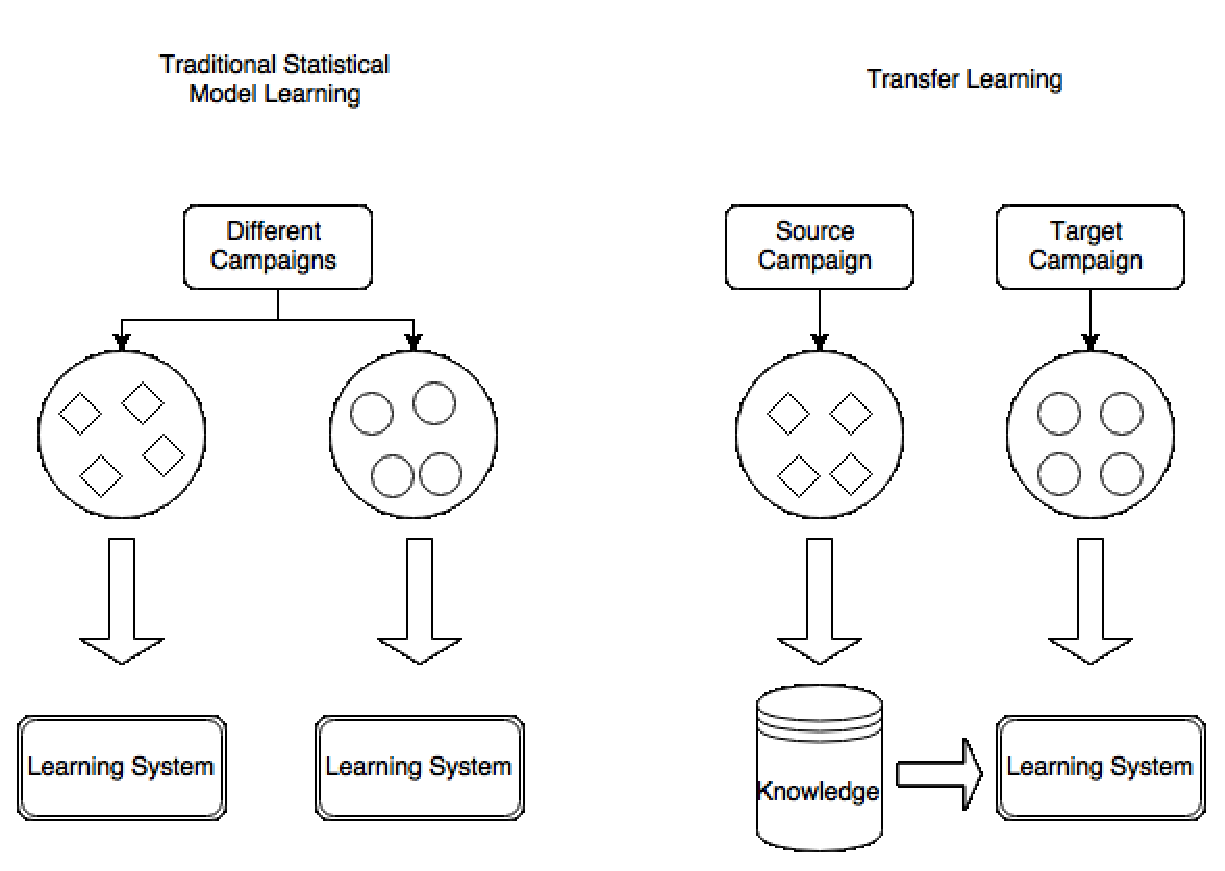
\includegraphics[width=\columnwidth]{transferlearning.eps}
\caption{Different Learning system between traditional machine learning and transfer learning}
\label{fig:transfer}
\end{figure}

At first, using the definitions in \cite{pan2010survey}, we specify \textit{domain} \textit{D} as each campaign's impressions raw data, and \textit{task} \textit{T} as the learning system of the model, in which, \(D = \{X,P(X)\}\), also  \(D = \{Y,P(Y|X)\}\). \(X = \{x_1,x_2, ..., x_n\}\) in which \(x_i\) is one impression in the campaign, and \(Y = \{y_1,y_2, ..., y_n\}\) is the label for each impression, namely whether in this impression the click occurs. The training data is composed of the pairs of \(\{x_i,y_i\}\) which can be used to train the model, and the conditional distribution \(P(Y|X)\). We define \textit{source domain} as the old campaign and \textit{target domain} as the new campaign, then \(X_s\) will be the feature space of source domain and \(P(X_s)\) is the marginal probability distribution of the feature space of source domain, similar, \(X_t\) will be the feature space of target domain and \(P(X_t)\) is the marginal probability distribution of the feature space of target domain. \(Y_s\) is the class label of the features in source domain and \(Y_t\) will be the corresponding label for target domain. By considering the relation between source domain and target domain, as well as source task and target task, the model learning problem can be classified as follows in the scope of online advertisement. 

\begin{enumerate}
\item if \(D_s = D_t\) and \(T_s = T_t\), this is a traditional machine learning problem. For example, the source and target advertisement campaigns follow the same distribution, and their learning tasks are the same, which are to predict the CTR based on the feature spaces. 

\item if  \(D_s \neq D_t\) and \(T_s = T_t\), which means the source and target domains are distinct but with the same tasks. The problem is also known as \textit{domain adaptation} \cite{arnold2007comparative} since the two domains are different in the marginal probability distribution but same for tasks. This situation can be further classified into two types:
    \begin{itemize}
    \item  \(X_s \neq X_t\), which means the feature spaces of the two domains are different with each other, for example, one domain of an advertisement campaign  \textit{International e-commerce} and the other is from \textit{ Software} as shown in \cite{zhang2014real}, if the impressions of the two domains are encoded into binary feature, surely there will be small overlap between the two feature spaces and the feature spaces will be largely different.
    \item \(P(X_s) \neq P(x_t) \), which means the probability distributions of the two advertisement campaigns are different, so they are from different fields, with different themes. 
    
    \end{itemize}
\item if  \(D_s = D_t\) and \(T_s \neq T_t\), it can also be classified into two types:
     \begin{itemize}
    \item  \(Y_s \neq Y_t\), this means the label spaces are different for two domains, as an example for online advertisement, the label in one domain could be click/non-click, which is dichotomic, but in the other domain the labels can be winning price, which is continuous.
    \item \(P(Y_s|X_s) \neq P(Y_t|X_t) \), this means the conditional probability distributions of the label on feature spaces are different for two domains, one example can be due to the existence of online robots, for one campaign all the impressions are randomly clicked or seen by programs, but the other campaign successfully prevent themselves from the robots so all clicks are effective and valid which simulates the human behaviors in the real world.  
  \end{itemize}
\end{enumerate}

In this paper, we will focus on transductive transfer learning, or \textit{domain adaptation}, since our learning task is obvious, which is CTR prediction, and we assumes that the robots are rare in the campaign, so the conditional probability are similar between the two campaigns, since the similar human behaviors will lead to similar advertisement clicking actions. 

As discussed above, domain is composed of feature space and feature probability distribution. In this paper, since our goal is to compare the performance of binary feature and counting feature, so we will represent the feature space and feature probability distribution of source and target domain in Table~\ref{tab:domainadapt}.

\begin{table}[h]
\centering
\begin{tabular}{ c | l | l }
Feature Types & Feature Space & Feature Distribution \\
\hline \hline
Binary Feature & Different & Different  \\
Counting Feature & Same & Different
\end{tabular}
\caption{Source and Target domain comparison for Binary and Counting Features}
\label{tab:domainadapt}
\end{table}

To clarify, for binary feature, suppose in the user dataset of online advertisement there is a categorical feature \textit{nationality}, with the value \textit{China}, \textit{UK}, \textit{USA}, etc. It is not surprising that the original field space will be blew up to hundreds of features which is the number of countries in the world, without pre-processing, we even cannot distinguish \textit{UK} from \textit{Great Britain}, which makes astronomical number of features with the increasing of new impressions. Microsoft claims that they have hundreds of millions features \cite{graepel2010web} for each training dataset, as we are already in the age of big data online advertisement, we can expect that the data volume will increase to the magnitude of hundred billion with hundred billion sparse discrete features. Even for our experiment, millions of features will arise from the dataset when the number of impressions reach 1 million. Therefore, the feature spaces are always distinct between the old campaigns and new campaigns. 

Therefore, in this part we will discuss on how to apply a classifier trained on the old advertising campaigns, or source domains for the use in the new campaigns, or target domain. Since the distribution between the features in the source domain and target domain are different, we expect that the more similar the two distributions are, the better performance the classifier trained on the source domain will have on the target domain. As we said above, we define a distribution of a domain as \(D\) on the instance set \(X\), which are different from domain to domain, however, the tasks are the same in multiple domains. So what we propose here is as follows:
\begin{itemize}
  \item \(D_s \neq D_t\), and \(X_s \neq X_t\). This is not surprising since for advertisement campaigns, normally there is not a huge overlap among the two domains.  
  \item \(T_s = T_t\) which means that the learning tasks are the same for the two domains.
\end{itemize}
Therefore, we will be faced up to the following three problems:
\begin{enumerate}
  \item How to measure the variance between two domains ? Namely how to find the relation between \(D_s\) and \(D_t\) and to say they can be regarded as the same ?
  \item Whether we can directly apply the classifiers learned from source domain to target domain ? Instead of using probit distribution to represent weights space and update the weights with the new come-in data as an active learning problem, as discussed in \cite{graepel2010web}, we hope to find a baseline that even though without updating the weights but directly using the old weights space, whether we can still obtain decent CTR prediction performance ? Namely whether we can regard \(Pr(y_s|x_s)\) as the same of \(Pr(y_t|x_t)\) considering that \(X_s \neq X_t\) ? 
\end{enumerate}



\section{Advertisement Campaign Datasets Shift}
In this part, we will discuss on the relation between the distributions among different domains. Normally, the relation between two domains can be represented using the indicators in 
\cite{shen2015effective}:
\begin{itemize}
\item Similarity : A score which looks at how similar
the two domains are. In terms of probability model.
\item Novelty : A score which the additional part generated from the target domain which does not exist in the source domain.
\end{itemize}
The relation can be shown in Figure ~\ref{fig:crossdomain}
\begin{figure}[h]
\centering
\includegraphics[width=\columnwidth]{crossdomain.png}
\caption{Similarity and Novelty in Source and Target Domains}
\label{fig:crossdomain}
\end{figure}
Intuitively, we know that the bigger the novelty is, the harder that we can apply our classifiers into the new campaign. So we should find a method to measure the similarity and novelty between two domains. 
\cite{bickel2009discriminative} proposes the concept of \textit{Covariate Shift}, which shows the case that distribution generating the new data to be tested varies from the distribution that generating the data used to train the model, therefore the new inputs used as predictors will change between training and testing stages. To simplify, \(P(X_s) \neq P(X_t)\).

In order to measure the covariate shift between domains, I devised a simple method to quickly detect the similarity and novelty, the basic idea is that, given two domains, if their feature distributions are nearly identical to each other, we would be hard to distinguish between them if we mix them together. On the other hand, when the distribution differ to each other, it will be capable to predict the label of the two domains. So a basic experiment is designed as follows:
\begin{itemize}
\item For the source domain, we remove its label of \textit{click}, but add a new label \textit{source} to each impression to show that the source domain is \textit{source} dataset.
\item For the target domain, we also remove its label for clicks but add a new label \textit{target} to show they belong to another dataset
\item Mix the two dataset together and use 10 fold cross validation method to train a model using a sample of the data and use the rest of the data as test to predict the label of dataset.
\item After 10 times of trial, for each pair of source and target domains, we can get the mean RMSE and regard it as the final RMSE between the two domains, the higher the RMSE, the harder that the classifiers to predict the label of the two datasets, showing that the two domains are hard to distinguish, and the distributions of them are more similar.
\item We use the idea proposed in \cite{ben2010theory}, as the \textit{transfer distance}, or \textif{Proxy-A-distance} (PAD) to measure how two domains are different to each other, the metric is defined as:
\begin{equation}
A distance = 2 \times (1-2 \times \epsilon)
\end{equation}
in which \(\epsilon\) is the generalization error of a classifier to distinguish the labels of the input data, here we use RMSE to represent it. So the lower the \textit{A-distance} is, the similar the two domains are.

Since we have 10 campaigns from the Adform dataset, for each dataset, we calculate its \textit{A-distance} with all other 9 campaigns to get a vector of 9 A-distance, and obtain the mean and variance value of this vector, the result is in Figure \ref{fig:beforeall}.

\end{itemize}
\begin{figure}[h]
\centering
\includegraphics[width=\columnwidth]{beforesigmoidall.png}
\caption{Mean and Variance value of A-distance sets of one campaign to the other 9 campaigns}
\label{fig:beforeall}
\end{figure}

From Figure ~\ref{fig:beforeall} we can see that the \textit{A-distance} are big and varies in a big range. Especially for counting feature the feature spaces of the 10 campaigns differ from each other dramatically. It is not surprising since counting feature is able to transfer the variability in the weights space to feature space, so the weights space of counting feature are much more similar to each other than binary feature. We can conclude from this part that \(Pr(x_s) \neq Pr(x_t)\)

\section{Cross Dataset Generalization}
The lucky thing is that based on the Bayesian format of logistic regression model,

\begin{equation}
Pr(y|x,w) = \frac{Pr(w|x,y)*Pr(y|x)}{Pr(w)}
\end{equation}

in which 
\begin{equation}
sigmoid = \frac{1}{1 + \exp(-w^T x)} 
\end{equation}

we can know that the inference of logistic regression is not based on \(Pr(x)\), but on \(Pr(y|x)\) largely. 

Then we can transform the feature space \(x\) into a new logistic space \(sigmoid(x^T*w)\) when \(y = 1\) which is as follows:



\begin{bmatrix} 
sigmoid(w_1*x_{11}) & sigmoid(w_1*x_{12}) .... & sigmoid(w_n * x_{1n})\\
sigmoid(w_1*x_{21}) & sigmoid(w_1*x_{22}) .... & sigmoid(w_n * x_{2n})\\
......\\
sigmoid(w_1*x_{N1}) & sigmoid(w_1*x_{N2}) .... & sigmoid(w_n * x_{Nn})
\end{bmatrix}

And using the same method as above, the similarities among the logistic spaces can be shown as follows:
\begin{figure}[h]
\centering
\includegraphics[width=\columnwidth]{aftersigmoid.png}
\caption{Mean and Variance value of A-distance sets of one campaign to the other 9 campaigns for y-space}
\label{fig:after1}
\end{figure}

It can be seen that in most cases the A-distance between the source domain to the rest of the targets domains are quite low, so \(Pr(y_s|x_s) = Pr(y_t|x_t)\) is a reasonable assumption.

Therefore, we can directly apply the model learned from old campaign to the new campaign and we are expected to still get decent CTR prediction performance, what's more, since the counting value of counting feature model can take over the variability between old and new campaigns, by updating the counting value, we can gradually transform the distribution of old campaign \(Pr(x_s)\) to \(Pr(x_t)\) with increasing number of new incoming data, thus outperforming binary feature considerably after several updates. 

\chapter{Experiment Results}
\label{chapterlabel7}

\subsection{Experiment Setup, Dataset Introduction and Measurement Method}

In this part, the results of two experiments will be shown. At first, we will represent that the performance of counting feature on non-linear regression model is comparable to that of one-hot binary feature of linear regression model. Secondly, we will show that counting feature performs significantly better than binary feature in cross-domain learning problem. 

For Cross Domain problem, we will do the experiment in the following scenario. An ad company serves for different clients for CTR prediction. Based on the information from old campaigns, it hopes to get accurate CTR prediction result for new campaigns without training new model but directly make use the off-the-shelf model derived from old campaigns. \vspace{5mm}

In this experiment, the whole 14 days dataset will be splitted based on the client id so that in each sub dataset all impressions are from a unique client. To simulate the real world situation that the ad data is not static but performs as a continuous data stream, the new campaign dataset will be further divided into smaller data capsules. Then on the one side, the old campaign dataset will be transformed into binary feature dataset then the model will be trained based on it. Then capsules will be sent into the model in sequence to estimate its CTR thus AUC for test dataset will be obtained. \vspace{5mm}

While on the other side, counting feature bears the advantage that its number of features are limited, and feature values are continuous. So unlike 0-1 binary feature, it is possible to update the feature values as more information from new campaign arrives with fixed model weights. The representation of two scenarios can be represented as follows in Figure ~\ref{fig:binary}

\begin{figure}[t]
\centering
\includegraphics[width=\columnwidth]{countingdiagram.png}
\caption{Estimate new campaign CTR using Binary Feature and Counting Feature Comparison}
\label{fig:binary}
\end{figure}




\subsection{Performance Comparison of Binary and Counting Feature in CTR prediction Problem}

In this section two experiments are conducted to compare the CTR prediction performance of Binary and Counting feature in terms of logistic regression and gradient boosting regression tree (GBRT) model. The first experiment is based on the public dataset from Ipinyou, which was released by the Chinese RTB company Ipinyou for global RTB algorithm competition in 2013. The dataset includes logs of ad auctions, bids, impressions, and also clicks \ref{zhang2014real}. All the features except for \textit{Usertag} are used in the experiment due to the bias in that feature. The result is as follows:





\begin{figure}[h]
\centering
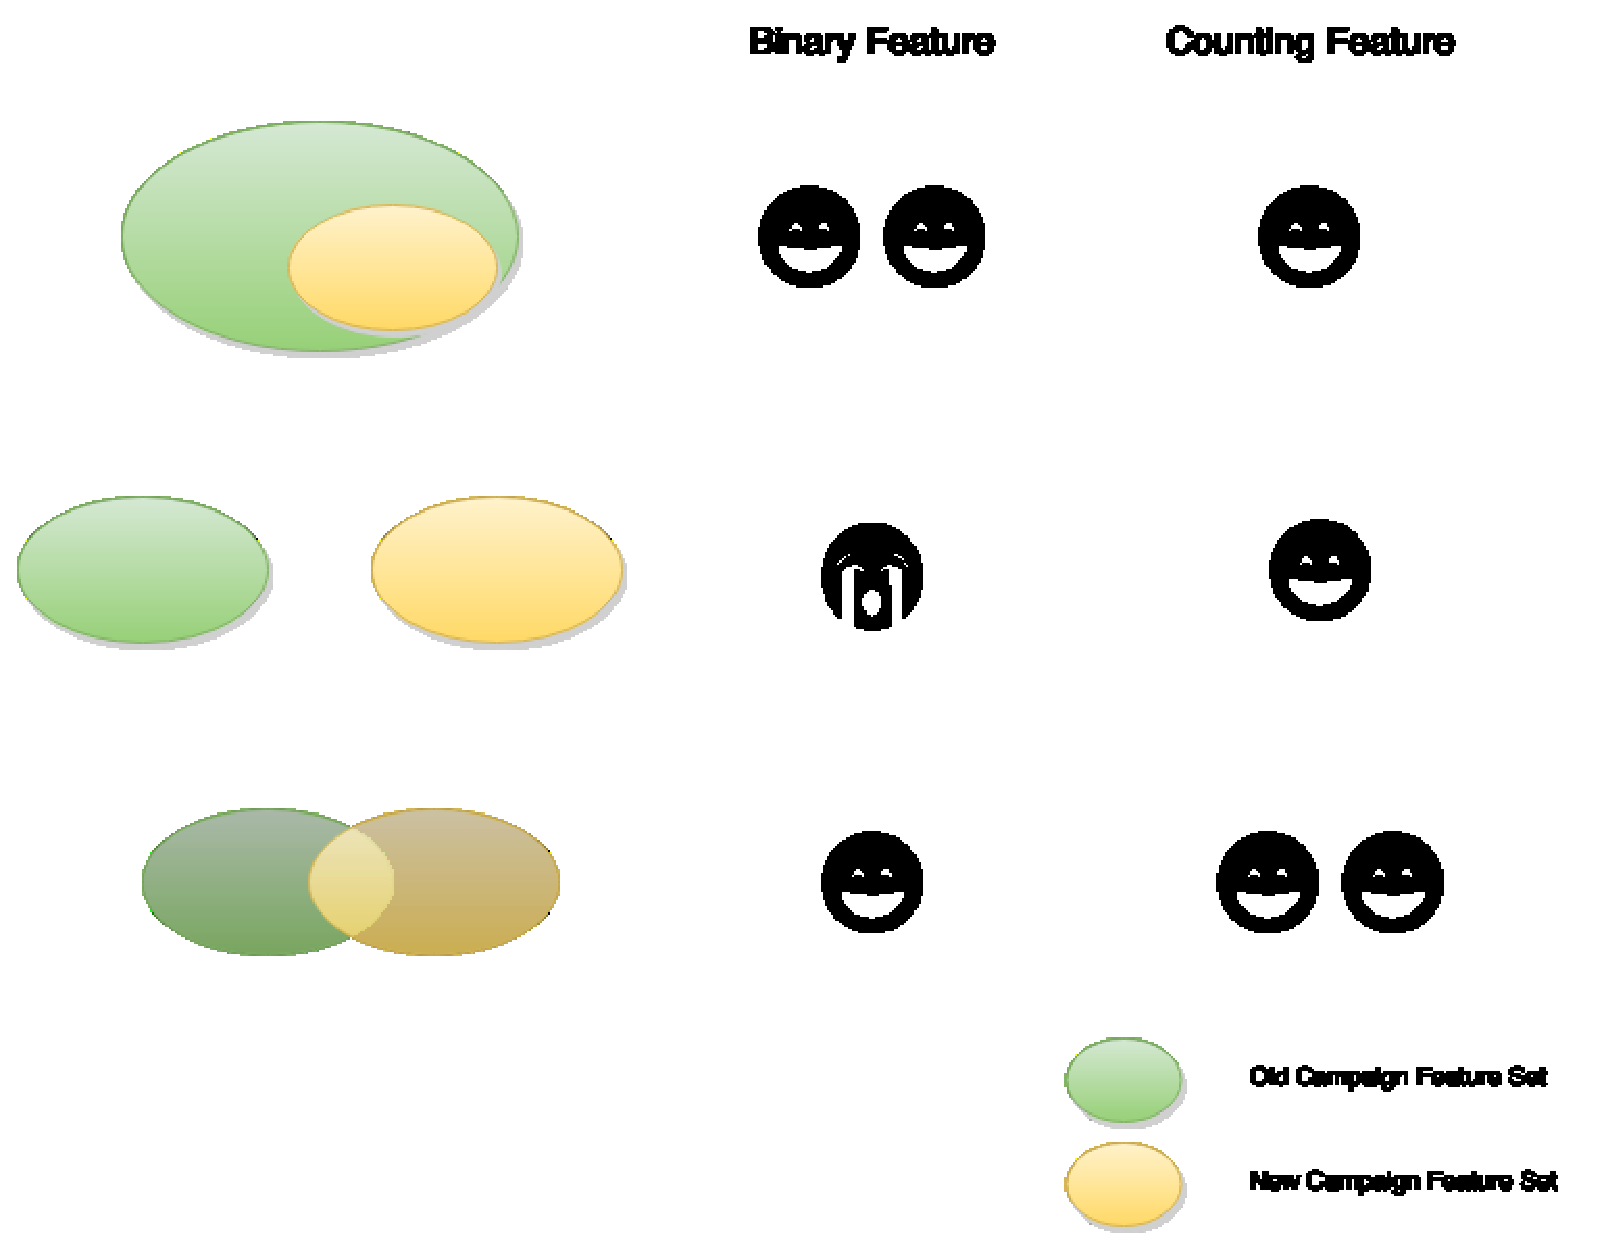
\includegraphics[width=\columnwidth]{Datasetbias.eps}
\caption{Three types of relation of feature sets between train dataset and test dataset}
\label{fig:datasetbias}
\end{figure}

\subsection{Performance Comparison of Binary and Counting Feature in Cold Start Problem}

In this part, the experiments will be done based on the dataset provided by a ad company in March which includes the data for 14 consecutive days, the dataset are separated by client id so that in each small dataset there are only the impressions from one unique client. In this experiment, the client with more than 500,000 impression are chosen so that 4 sub datasets are obtained which are from distinct clients. The detail of the four clients are shown in Table~\ref{tab:campainid}.


\begin{table}[t]
\centering
\begin{tabular}{c | c | c | c }
· 
\end{tabular}
\caption{Statistical Information of top 10 advertisement clients}
\label{tab:campainid}
\end{table}

\iffalse
\begin{table}[t]
 \centering
 \begin{tabular}{ ||c c || } 
 \hline
 Client id  & Number \\
 \hline
 20762 & 1068606 \\ 
  15140 & 764355 \\ 
   1371 & 576709 \\ 
   12482 & 557120\\
 \hline
 \end{tabular}
 \caption{Four Biggest clients}
 \label{tab:campainid}
 \end{table}
 
\fi

The figure above shows the truth that dataset significantly decide upper bound of the accuracy to predict CTR. above performance comparison of binary feature and counting feature on CTR estimation reveals that performance of counting feature using non-linear regression model is comparable to that of binary feature using linear regression model, the precondition is that the training and test dataset share most of the features. However, in real world we will always be faced up with the situation that the information is unbalanced in train and test dataset. We define \textit{Feature Set} as a criterion to measure the information obtained in the dataset, which is represented by  \(S_i(f)\), in which \(f\) are the unique features in the dataset \(i\).\vspace{5mm}

The relation of the feature sets in dataset \(i\) and \(j\) can be catogrized into three types, in which \(i\) is the test dataset, and \(j\) is the training dataset, as shown in Figure~\ref{fig:datasetbias}.:
\begin{itemize}
\item When \(s_i \subset s_j\), the binary feature should perform better than counting feature in terms of CTR estimation. Since in this way all the feature information needed by test dataset is inclusive in training dataset, the model contains all the infomraiton as a general model, as with the above conclusion when both using linear logistic regression, binary feature is superior to counting feature.  
\item When \(s_i \cap s_j \equiv 0\), the counting feature should perform better than binary feature which degenerates into random algorithm. The reason is that there is no overlap between \(s_i\) and \(s_j)\), so all feature information in test dataset will be regared as \textit{other} for model derived from training dataset. However, for counting feature, this deficiency can be made up with the gradual increasing information of the dataset distribution. The counting value to some extent represents the feature distribution so when we assume that the train and test dataset share similar feature value distribution counting feature can still perform rather well while at same time prediction using binary feature is totoally impossible.
\item When \(s_i \cap s_j \neq 0\), the feature informaiton at this time is shared by train and test dataset. We define \textit{General Information} as the information shared by all the advertisement campaigns, and \textit{Specific Information} as the unique feature information owned by each of the campaign. In this situation, both binary feature and counting feature performs well granted that train and test dataset share enough feature information so that the model to some extent is universal among datasets. However, the upper-bound of performance of binary feature is around the AUC result of the CTR prediction for first data capsule in the data stream assuming the distribution among test dataset is identical, conversely, that is the lower-bound of the performance of counting feature since with the increasing of test instances, counting value will tend towards the real distribution of test dataset to compensate of the unbalanced counting weights value. 
\end{itemize}



\begin{figure}[t]
\centering
\includegraphics[width=\columnwidth]{coldstart_first.eps}
\caption{Performance Comparison of Binary and Counting feature for Cross Domain Learning before Counting Value Updating}
\label{fig:coldstart_first}
\end{figure}

\begin{figure}[t]
\centering
\includegraphics[width=\columnwidth]{coldstart.eps}
\caption{Performance Comparison of Binary and Counting feature for Cross Domain Learning after convergence}
\label{fig:coldstart}
\end{figure}

\begin{figure}[t]
\centering
\includegraphics[width=\columnwidth]{coldstartimprove.eps}
\caption{Performance Comparison of Binary and Counting feature for Cross Domain Learning after convergence}
\label{fig:coldstartimprove}
\end{figure}

Figure \ref{fig:coldstart_first} shows the comparison of the performance between binary feature and counting feature before updating counting values. As shown in the diagram above, for binary feature the counting value will be updated between 0 and 1 since it is discrete, however, because the values of counting feature is continuous, so it is possible to update its values with the introduction of new data from new campaign. Figure \ref{fig:coldstart_first} shows the fact that just after training the model from old campaign, directly using it to predict the CTR of new campaign, binary and counting features are suffering from the same bad performance. 

Figure \ref{fig:coldstart} shows the fact that counting feature indeed improve the performance of CTR prediction after a few times updating until convergence. After getting information from the new coming data, the counting value will be changed to represent the distribution of the new campaign somehow, which takes over the responsibility from the binary weights space. However for binary feature since its feature space is fixed so changing between 0 and 1 cannot represent the distribution of the new campaign so there is no performance improvement for binary feature after the updating. 

Figure \ref{fig:coldstartimprove} demonstrates the conclusion in last above well. If we assume that the distribution of the new campaign is identical, the performance of the CTR prediction in terms of AUC should be the same among all sub-dataset of the new campaign. We define  \(AUC_{\text{before}}\) as the CTR prediction performance for the first capsule of new campaign data, when there is no counting value update from new campaign and we can only predict it based on the model from the old campaign. We also define \(AUC_{\text{after}}\) as the peformance of binary or counting feature after all the information of the new campaign has been obtained by the model and it becomes converged. In Figure \ref{fig:coldstartimprove} we compare the\({AUC_{\text{after}}}/{AUC_{\text{before}}}\)
for binary feature and counting feature.From the plot it shows that for binary feature there is no improvement for most cases since the value is around 1 and for counting feature the improvement is high. 



Figure \ref{fig:matrixbefore} \ref{fig:matrixafter} and \ref{fig:matriximprove} shows the details of the result.In Figure \ref{fig:matrixbefore} we calculate \((AUC_{\text{before(count)}} - AUC_{\text{before(bi)}}) / AUC_{\text{before(bi)}} \) to show how counting feature improves the performance compared to binary feature before updating the counting values, the result shows that counting feature performs bad which is not surprising. 

In Figure \ref{fig:matrixafter} we shows the same calculating for that but after updating the counting values.  \((AUC_{\text{after(count)}} - AUC_{\text{after(bi)}}) / AUC_{\text{after(bi)}} \) is shown in the matrix. Green shows that the counting feature performs better than binary feature, and the percentage value shows by how many percents do the counting feature obtains in terms of CTR AUC performance. It shows that excluding the diagonal in which the train and test dataset are the same, so the binary feature should perform better than counting feature, In 61 out of 90 experiments counting feature performs better than binary feature, which is much better than we can see in Matrix \ref{fig:matrixbefore}.

Figure \ref{fig:matriximprove} calculates 
\((AUC_{\text{after(count)}}/AUC_{\text{before(count)}} -AUC_{\text{after(bi)}}/AUC_{\text{before(bi)}})  / (AUC_{\text{after(bi)}}/AUC_{\text{before(bi)}})  \), which shows that after updating the counting value, whether counting feature gains more performance improvement than binary feature, result shows that counting feature indeed improves much more than binary feature whose upper bound of CTR estimation is decided when the first subset of data comes. 

\begin{figure}[t]
\centering
\includegraphics[width=\columnwidth]{matrixbefore.eps}
\caption{Percentage of Performance Improvement of Counting Feature to Binary Feature in Cross Domain Learning before Counting Value Updating}
\label{fig:matrixbefore}
\end{figure}

\begin{figure}[t]
\centering
\includegraphics[width=\columnwidth]{matrixafter.eps}
\caption{Percentage of Performance Improvement of Counting Feature to Binary Feature in Cross Domain Learning After Convergence}
\label{fig:matrixafter}
\end{figure}

\begin{figure}[t]
\centering
\includegraphics[width=\columnwidth]{matriximprove.eps}
\caption{Percentage of Performance Improvement of Counting Feature Compared to Binary Feature}
\label{fig:matriximprove}
\end{figure}


\begin{figure}[t]
\centering
\includegraphics[width=\columnwidth]{variance.eps}
\caption{Cross-validation of binary and counting feature dataset mean and variance}
\label{fig:variance}
\end{figure}

\begin{figure}[t]
\centering
\includegraphics[width=\columnwidth]{2261.eps}
\caption{Performance 2261}
\label{fig:2261}
\end{figure}

\begin{figure}[t]
\centering
\includegraphics[width=\columnwidth]{2997.eps}
\caption{Performance 2997}
\label{fig:2997}
\end{figure}

\begin{figure}[t]
\centering
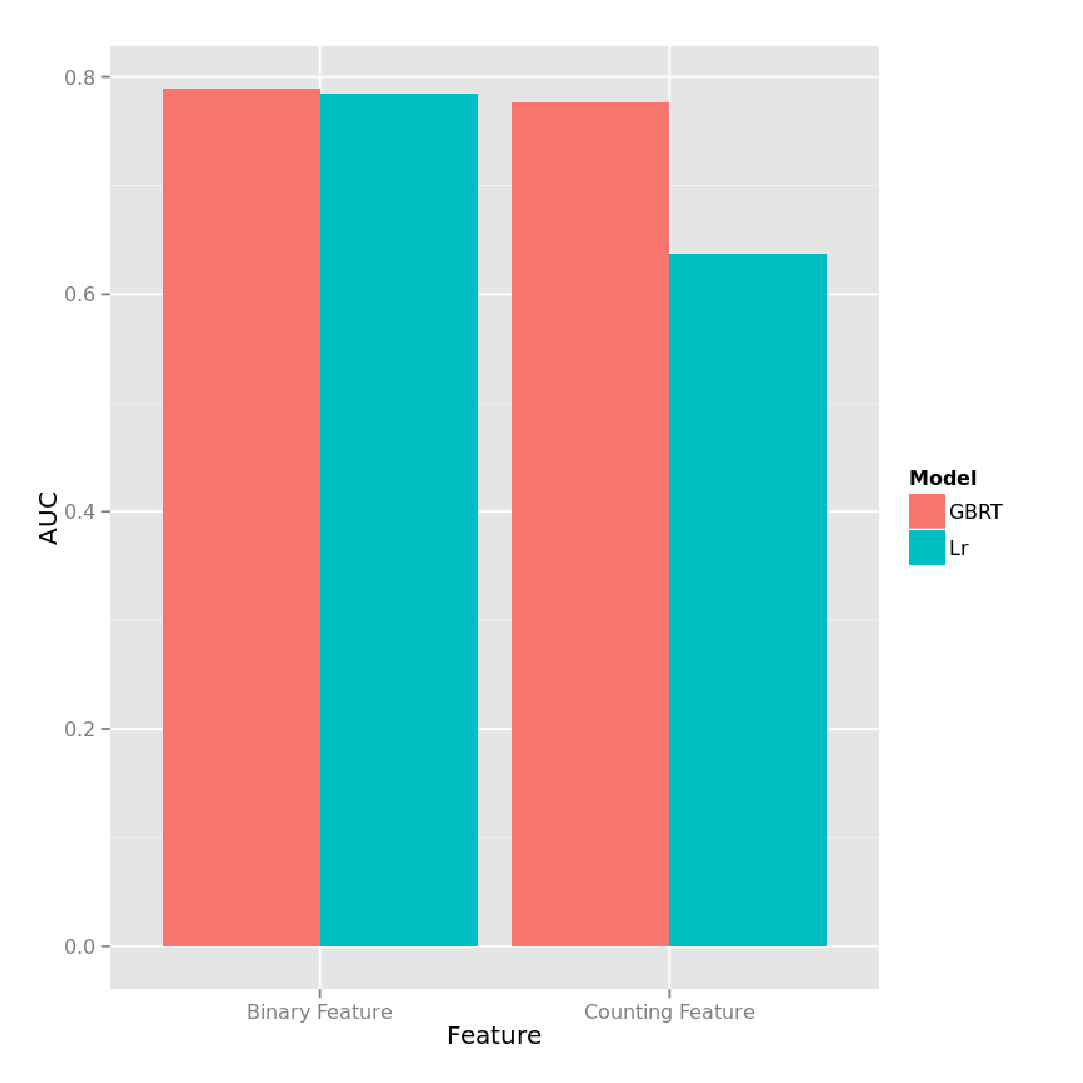
\includegraphics[width=\columnwidth]{3386.eps}
\caption{Performance 3386}
\label{fig:3386}
\end{figure}


% The data from 3-14 to 3-27 are regarded as training dataset, the data from 5- are regarded as test dataset, the count of training dataset is, test dataset is ~\ref{tab:campainid}

% \begin{table*}[h]
% \centering
% \begin{tabular}{ |c|c|c|c| } 
% \hline
% Shared Campaign  & Unique Train Dataset Campaign & Unique Test Dataset Campaign \\
% \hline
% 1310190 & 1307617, 884194, 1283235, 1335301  & 1466432, 1448738 \\ 
% & 1385319, 1349577, 1276074, 1363723 & 1406405, 1424966 \\ 
% &  1357245, 1341802, 1341937, 1307838 & 1424330, 1445998 \\ 
% &  1285558, 1358167, 1305663, 1299899 & 1458704, 1454382 \\
% &  1363711, 1386205, 1368830, 1366271 &  1472727, 1452138 \\
% \hline
% \end{tabular}
% \label{tab:campainid}
% \end{table}

% Only the instances from the campaign with more than 500 clicks and 50000 impressions will be remained, the campaigns can be classified as the ones shared by the training and test dataset, the ones unique to training dataset and the one unique to test dataset.  

% \(1/3\) of the training dataset is used as train dataset, \(2/3\) will be used as count dataset. In order to increase the generalization of training dataset to improve the universality of the trained prediction model, four campaign will constitute one training dataset and two campaigns are used to make up a test dataset to decrease the bias of test dataset.  

% For the sake of convenience, the training dataset will be labeled as 1,2,3,4 and 5, from top to the bottom, as well as the test dataset. For each training dataset, the prediction model will be build based on it which will be used to test the data stream from each of the test dataset, the result is in 6.3.


\begin{figure*}
    \centering
    \begin{subfigure}[b]{0.3\textwidth}
        \centering
        \includegraphics[width=\textwidth]{cos}
        \caption{Cos Similarity Comparison Between Pairwise of Binary Feature and Counting Feature}
        \label{fig:cos}
    \end{subfigure}
    \hfill
    \begin{subfigure}[b]{0.3\textwidth}
        \centering
        \includegraphics[width=\textwidth]{correlation}
        \caption{Correlation Similarity Comparison Between Pairwise of Binary Feature and Counting Feature}
        \label{fig:correlation}
    \end{subfigure}
    \hfill
    \begin{subfigure}[b]{0.3\textwidth}
        \centering
        \includegraphics[width=\textwidth]{euclidean}
        \caption{Euclidean Distance Comparison Between Pairwise of Binary Feature and Counting Feature}
        \label{fig:euclidean}
    \end{subfigure}
    \caption{Comparison of Binary and Counting Feature Model Weights Space}
    \label{fig:three graphs}
\end{figure*}


Figure \ref{fig:variance} shows that the variance and mean for binary and counting feature dataset are nearly the same. 

Figure \ref{fig:three graphs} shows that the similarity among weights space for counting feature is higher than counting feature. 



\iffalse
Experiment 1.1: Training Dataset  (20762), Test Dataset  (15140) in Figure~\ref{fig:fig1}.:
\begin{figure}[h]
\centering
\includegraphics[width=\columnwidth]{20762_15140.eps}
\caption{Training Dataset  (20762), Test Dataset  (15140)}
\label{fig:fig1}
\end{figure}

Experiment 1.2: Training Dataset  (20762), Test Dataset  (1371) in Figure~\ref{fig:fig2}.:
\begin{figure}[h]
\centering
\includegraphics[width=\columnwidth]{20762_1371.eps}
\caption{Training Dataset  (20762), Test Dataset  (1371)}
\label{fig:fig2}
\end{figure}

Experiment 1.3: Training Dataset  (20762), Test Dataset  (12482) in Figure~\ref{fig:fig2}.:
\begin{figure}[h]
\centering
\includegraphics[width=\columnwidth]{20762_12482.eps}
\caption{ Training Dataset  (20762), Test Dataset  (12482)}
\label{fig:fig2}
\end{figure}

Experiment 2.1: Training Dataset  (15140), Test Dataset  (20762) in Figure~\ref{fig:fig3}.:
\begin{figure}[h]
\centering
\includegraphics[width=\columnwidth]{15140_20762.eps}
\caption{Training Dataset  (15140), Test Dataset  (20762)}
\label{fig:fig3}
\end{figure}

Experiment 2.2: Training Dataset  (15140), Test Dataset  (1371) in Figure~\ref{fig:fig4}.:
\begin{figure}[h]
\centering
\includegraphics[width=\columnwidth]{15140_1371.eps}
\caption{Training Dataset  (15140), Test Dataset  (1371)}
\label{fig:fig4}
\end{figure}

Experiment 2.3: Training Dataset  (15140), Test Dataset  (12482) in Figure~\ref{fig:fig5}.:
\begin{figure}[h]
\centering
\includegraphics[width=\columnwidth]{15140_12482.eps}
\caption{Training Dataset  (15140), Test Dataset  (12482) }
\label{fig:fig5}
\end{figure}

Experiment 3.1: Training Dataset  (1371), Test Dataset  (20762) in Figure~\ref{fig:fig6}.:
\begin{figure}[h]
\centering
\includegraphics[width=\columnwidth]{1371_20762.eps}
\caption{ Training Dataset  (1371), Test Dataset  (20762)}
\label{fig:fig6}
\end{figure}

Experiment 3.2: Training Dataset  (1371), Test Dataset  (15140) in Figure~\ref{fig:fig7}.:
\begin{figure}[h]
\centering
\includegraphics[width=\columnwidth]{1371_15140.eps}
\caption{Training Dataset  (1371), Test Dataset  (15140)}
\label{fig:fig7}
\end{figure}

Experiment 3.3: Training Dataset  (1371), Test Dataset  (12482) in Figure~\ref{fig:fig8}.:
\begin{figure}[h]
\centering
\includegraphics[width=\columnwidth]{1371_12482.eps}
\caption{Training Dataset  (1371), Test Dataset  (12482)}
\label{fig:fig8}
\end{figure}

Experiment 4.1: Training Dataset  (12482), Test Dataset  (20762) in Figure~\ref{fig:fig9}.:
\begin{figure}[h]
\centering
\includegraphics[width=\columnwidth]{12482_20762.eps}
\caption{Training Dataset  (12482), Test Dataset  (20762)}
\label{fig:fig9}
\end{figure}

Experiment 4.2: Training Dataset  (12482), Test Dataset  (1371) in Figure~\ref{fig:fig10}.:
\begin{figure}[h]
\centering
\includegraphics[width=\columnwidth]{12482_1371.eps}
\caption{Training Dataset  (12482), Test Dataset  (1371)}
\label{fig:fig10}
\end{figure}

Experiment 4.2: Training Dataset  (12482), Test Dataset  (15140) in Figure~\ref{fig:fig11}.:
\begin{figure}[h]
\centering
\includegraphics[width=\columnwidth]{12482_15140.eps}
\caption{Training Dataset  (12482), Test Dataset  (15140)}
\label{fig:fig11}
\end{figure}

\fi



\chapter{Conclusions and Future Work}
\label{conclusion}
In this project, we introduce the concept of \textit{counting feature} which is composed of \textit{frequency feature} and \textit{average CTR feature}, and prove that for the same dataset, counting feature space is a non-linear transformation of binary feature space, and the CTR prediction performance in terms of AUC of counting feature using GBRT algorithm is comparable to that of binary feature using linear logistic regression model. Unlike previous and current researches which focus more on the improvement of machine learning model and algorithm in CTR prediction problem, we turn to the more fundamental, but more crucial to the industry, research field, which is feature engineering. We show that counting feature can not only transform the extremely high dimension feature space into low, scalable, interpretable space, but also remain the comparable CTR prediction performance as traditional method, which will largely decrease the memory and time cost for industry. 

To the best of our knowledge, our work is the first one to systematically research on statistical feature, namely counting feature, even though statistical feature has been used by a small range of companies in daily business, our work is the first one to not only provide experimental result, but also mathematical derivation. The most important thing is, we present that counting feature can partly solve the classical \textit{cold start} problem to extend the knowledge from one advertising campaign to the others, we show that without updating old model parameters we can still obtain high performance using counting feature in the context of \textit{cross-domain learning} problem. There are few literature studying on cross-domain learning problem in the field of online advertising, and we are the first one with simplest implementation and solid backups.

However, the research in of our work is not ended. Firstly, we need more dataset to test our theory since currently we only have two datasets which are from iPinYou and Adform, also more linear and non-linear machine learning algorithms should be used to validate the correctness of our theory. Secondly, now we can only do the offline experiment, however, since for cross-learning problem, commonly the new income data should be in the format of stream, we already mimic the process of data stream, but implementing the experiment online will be absolutely what we will do next. Lastly, for the cross-learning problem, now we assume that the marginal distribution of the joint probability distribution of feature and label space are the same so that directly using model from old campaign to new ones is feasible, however, the covariate or domain shift is inevitable in the real world machine learning problem, a multitask optimization method to not only minimise the different between the feature distribution of source and target campaign, but also classifier difference should be studied to increase the CTR prediction further.

%\addcontentsline{toc}{chapter}{Appendices}

% The \appendix command resets the chapter counter, and changes the chapter numbering scheme to capital letters.
%\chapter{Appendices}
\appendix
\chapter{List of Code}
\label{appendixlabel1}
1. Make Feature \\
(1). Make Binary Feature
\lstset{language=Python, 
        basicstyle=\ttfamily\small, 
        keywordstyle=\color{blue},
        commentstyle=\color{comments},
        stringstyle=\color{black},
        showstringspaces=false,
        identifierstyle=\color{black}}
\begin{lstlisting}[numbers=left, breaklines=true]
import pandas as pd
import sys
import numpy as np
import operator
import random
from collections import Counter
from math import sqrt
from random import shuffle
import math
def getsecondfeature(frame_train_count):
    columns1= ['log_date', 'log_time_hour', 'client_id', 'placement_id', \\
    'inventory_source_id', 'url', 'position_id', 'size', 'browser_id', \\
'os_id', 'user_agent', 'screen_size_id', 'visited_domains', 'visited_logpoints', 'clicker']
    count_valid = {}
    second = {}
    second_valid = {}
    second_whole = []

    for idx1, val1 in enumerate(columns1):
        for idx2, val2 in enumerate(columns1[idx1+1:]):
            second[val1] = frame_train_count.groupby([val1, val2])\\
            [val1].count()
            second_valid[val1] = [key for key in second[val1].keys() if \\
            second[val1][key] > 10000]
            second_whole.extend(second_valid[val1])
            second_whole.append(val1+':other')\\
    return second_whole

def notlast(itr):
    itr = iter(itr)  # ensure we have an iterator
    prev = itr.next()
    for item in itr:
        yield prev

        prev = item
print 'start'
file = sys.argv[1]
file = int(float(file))
cnt = Counter()
ctrcount = Counter()
pd.options.display.float_format = '{:.25f}'.format

columns = ['log_date', 'log_time_hour',
           'inventory_source_id', 'position_id', 'size', 'browser_id', 'os_id', 'user_agent',
           'screen_size_id', 'visited_domains', 'visited_logpoints', 'clicker', 'click_count']

columns1= ['log_date', 'log_time_hour', 'client_id', 'placement_id',
           'inventory_source_id', 'domain', 'url', 'position_id', 'size', 'browser_id', 'os_id', 'user_agent',
           'screen_size_id', 'visited_domains', 'visited_logpoints', 'clicker']

path_train_train = '%d/train.train.txt' % file
path_train_count = '%d/train.count.txt' %file
path_test_test = '%d/test.test.txt' % file
path_test_valid = '%d/test.valid.txt' % file

fo_train = open('%d/train.bi.txt' %file, 'w')
fo_test_test = open('%d/test.bi.test.txt' % file, 'w')
fo_test_valid = open('%d/test.bi.valid.txt' % file, 'w')
fo_index = open('%d/index.txt' % file, 'w')

frame_train_train = pd.read_csv(path_train_train,dtype=str,\\
error_bad_lines = False)
frame_train_count = pd.read_csv(path_train_count,dtype=str,\\
error_bad_lines = False)
frame_test_test = pd.read_csv(path_test_test,dtype=str,\\
error_bad_lines = False)
frame_test_valid = pd.read_csv(path_test_valid,dtype=str,\\
error_bad_lines = False)
total_length = len(frame_train_count)
dict_unique = {}

length = 0
frame_train_count = pd.DataFrame(frame_train_count, columns=columns)

for c_index in range(0, len(columns) - 1):
    seri_train_count = frame_train_count.ix[1:len(frame_train_count)-1,\\
    c_index]

    seri_train_count = seri_train_count[~seri_train_count.isnull()]
    unique_s = seri_train_count.unique()
    unique_s = unique_s.tolist() + ['other']
    index = 0
    unique_list = []
    dict_u = {}
    for u in range(0, len(unique_s)):
        dict_u[unique_s[u]] = u + length
    dict_unique[columns[c_index]] = dict_u
    length = length + len(unique_s)
index = 0
record_length = 0
for column in notlast(columns):
    index = index + 1
    dict_u = dict_unique[column]
    record_length = record_length + len(dict_u)
    for key in dict_u:
        fo_index.write(str(index) + ':' + str(key) + ' ' + str(dict_u[key]))
        fo_index.write('\n')
record_length = record_length + 100
record_length = 2155314

        # ctr[column] = (frame_train_ctr.groupby(column).size()/float(count[column])).fillna(0)
for index, row in frame_train_train.iterrows():
    if row[-1] == str(0) or row[-1] == 0:
        fo_train.write(str(0))
    else:
        fo_train.write(str(1))

    for column in notlast(columns):
        dict_u = dict_unique[column]
        if row[column] not in dict_u:
            id = dict_u['other']
            fo_train.write(' ' + str(id) + ':' + str(1))
        else:
            id = dict_u[row[column]]
            fo_train.write(' ' + str(id) + ':' + str(1))

    fo_train.write('\n')
fo_train.close()

for index, row in frame_test_test.iterrows():
    if row[-1] == str(0) or row[-1] == 0:
        fo_test_test.write(str(0))
    else:
        fo_test_test.write(str(1))

    for column in notlast(columns):
        dict_u = dict_unique[column]
        if row[column] not in dict_u:
            id = dict_u['other']
            fo_test_test.write(' ' + str(id) + ':' + str(1))
        else:
            id = dict_u[row[column]]
            fo_test_test.write(' ' + str(id) + ':' + str(1))

    fo_test_test.write('\n')
fo_test_test.close()

\end{lstlisting}
(2) Make Counting Feature
\lstset{language=Python, 
        basicstyle=\ttfamily\small, 
        keywordstyle=\color{blue},
        commentstyle=\color{comments},
        stringstyle=\color{black},
        showstringspaces=false,
        identifierstyle=\color{black}}
\begin{lstlisting}[numbers=left, breaklines=true]
import pandas as pd
import sys
import operator
import random
from collections import Counter
from math import sqrt
from random import shuffle
import math
import matplotlib.pyplot as plt
import numpy as np

def notlast(itr):
    itr = iter(itr)  # ensure we have an iterator
    prev = itr.next()
    for item in itr:
        yield prev
        prev = item
def median(mylist):
    sorts = sorted(mylist)
    length = len(sorts)
    if not length % 2:
        return (sorts[length / 2] + sorts[length / 2 - 1]) / 2.0
    return sorts[length / 2]

def k_means(data_pts, k=None):
    """ Helper functions """

    def lists_are_same(la, lb):  # see if two lists have the same elements
        out = False
        for item in la:
            if item not in lb:
                out = False
                break
            else:
                out = True
        return out

    def distance(a, b):  # distance between (x,y) points a and b
        return sqrt(abs(a[0] - b[0]) ** 2 + abs(a[1] - b[1]) ** 2)

    def average(a):  # return the average of a one-dimensional list (e.g., [1, 2, 3])
        return sum(a) / float(len(a))

    """ Set up some initial values """
    if k is None:  # if the user didn't supply a number of means to look for, try to estimate how many there are
        n = len(data_pts)  # number of points in the dataset
        k = int(sqrt(n / 2))  # number of clusters - see
        #   http://en.wikipedia.org/wiki/Determining_the_number_of_clusters_in_a_data_set#Rule_of_thumb
    if k < 1:  # make sure there's at least one cluster
        k = 1

    """ Randomly generate k clusters and determine the cluster centers,
        or directly generate k random points as cluster centers. """

    init_clusters = data_pts[:]  # put all of the data points into clusters
    shuffle(init_clusters)  # put the data points in random order
    init_clusters = init_clusters[0:k]  # only keep the first k random clusters

    old_clusters, new_clusters = {}, {}
    for item in init_clusters:
        old_clusters[item] = []  # every cluster has a list of points associated with it. Initially, it's 0

    while 1:  # just keep going forever, until our break condition is met
        tmp = {}
        for k in old_clusters:  # create an editable version of the old_clusters dictionary
            tmp[k] = []

        """ Associate each point with the closest cluster center. """
        for point in data_pts:  # for each (x,y) data point
            min_clust = None
            min_dist = 1000000000  # absurdly large, should be larger than the maximum distance for most data sets
            for pc in tmp:  # for every possible closest cluster
                pc_dist = distance(point, pc)
                if pc_dist < min_dist:  # if this cluster is the closest, have it be the closest (duh)
                    min_dist = pc_dist
                    min_clust = pc
            tmp[min_clust].append(point)  # add each point to its closest cluster's list of associated points

        """ Recompute the new cluster centers. """
        for k in tmp:
            associated = tmp[k]
            xs = [pt[0] for pt in associated]  # build up a list of x's
            ys = [pt[1] for pt in associated]  # build up a list of y's
            x = average(xs)  # x coordinate of new cluster
            y = average(ys)  # y coordinate of new cluster
            new_clusters[(
            x, y)] = associated  # these are the points the center was built off of, they're *probably* still associated

        if lists_are_same(old_clusters.keys(), new_clusters.keys()):  # if we've reached equilibrium, return the points
            return old_clusters.keys()
        else:  # otherwise, we'll go another round. let old_clusters = new_clusters, and clear new_clusters.
            old_clusters = new_clusters
            new_clusters = {}

file = sys.argv[1]
file = int(float(file))
cnt = Counter()
ctrcount = Counter()
count = {}
ctr = {}
test_count = {}
pd.options.display.float_format = '{:.25f}'.format

columns = ['log_date', 'log_time_hour',
           'inventory_source_id', 'position_id', 'size', 'browser_id', 'os_id', 'user_agent',
           'screen_size_id', 'visited_domains', 'visited_logpoints', 'clicker', 'click_count']

path_train_train = '%d/train.train.txt' % file
path_train_count = '%d/train.count.txt' % file
path_test_test = '%d/test.test.txt' % file
path_test_valid = '%d/test.valid.txt' % file

fo_train = open('%d/train.countfeature.txt' % file, 'w')
fo_test_test = open('%d/test.countfeature.test.txt' % file, 'w')
fo_test_valid = open('%d/test.countfeature.valid.txt' % file, 'w')
fo_index = open('%d/index_count.txt' % file, 'w')
fo_count_index = open('%d/index_countfeature.txt' % file, 'w')

index = 0
for column in notlast(columns):

    fo_count_index.write(column + ':' + 'frequency' + ' ' + str(index))
    index = index + 1
    fo_count_index.write('\n')
    fo_count_index.write(column + ':' + 'averagectr' + ' ' + str(index))
    index = index + 1
    fo_count_index.write('\n')

#print 'start'
frame_train_train = pd.read_csv(path_train_train, dtype=str,error_bad_lines = False)
frame_train_count = pd.read_csv(path_train_count, dtype=str,error_bad_lines = False)
frame_test_test = pd.read_csv(path_test_test, dtype=str,error_bad_lines = False)
frame_test_valid = pd.read_csv(path_test_valid, dtype=str,error_bad_lines = False)
total_length = len(frame_train_count)
test_total_length = len(frame_test_test)

for column in columns:
    count[column] = frame_train_count.groupby(column).size()
    test_count[column] = frame_test_test.groupby(column).size()

frame_train_ctr = frame_train_count[(frame_train_count.click_count == str(1))]
aver_count = {}
aver_ctr = {}

index = 1
for column in notlast(columns):
    count[column] = count[column].astype(float)
    #ctr[column] = math.log10((frame_train_ctr.groupby(column).size() / count[column]).fillna(0) + math.pow(10, -100))
    ctr[column] = ((frame_train_ctr.groupby(column).size() / count[column]).fillna(0))

    test_count[column] = test_count[column].astype(float)/float(test_total_length)
    count[column] = count[column].astype(float)/float(total_length)

    l = count[column].values.tolist()
    lctr = ctr[column].values.tolist()
    if len(l) == 0:
        aver_count[column] = 0

    else:
        aver_count[column] = sum(l)/float(len(l))
    if len(lctr) == 0:
        aver_ctr[column] = 0

    else:
        aver_ctr[column] = sum(lctr)/float(len(lctr))
        
# ctr[column] = (frame_train_ctr.groupby(column).size()/float(count[column])).fillna(0)
for index, row in frame_train_train.iterrows():
    id = 0
    if row[-1] == str(0) or row[-1] == 0:
        fo_train.write(str(0))
    else:
        fo_train.write(str(1))

    for column in notlast(columns):

        if column != 'click_count':

            if row[column] in count[column]:
                fo_train.write(' ' + str(id) + ':' + str(count[column][row[column]]))
                id = id + 1
                fo_train.write(' ' + str(id) + ':' + str(ctr[column][row[column]]))
                id = id + 1
            else:


                fo_train.write(' ' + str(id) + ':' + str(aver_count[column]))
                id = id + 1
                fo_train.write(' ' + str(id) + ':' + str(aver_ctr[column]))
                id = id + 1
    fo_train.write('\n')

fo_train.close()

for index, row in frame_test_test.iterrows():

    id = 0
    if row[-1] == str(0) or row[-1] == 0:
        fo_test_test.write(str(0))
    else:
        fo_test_test.write(str(1))

    for column in notlast(columns):

        if column != 'click_count':

            if row[column] in count[column]:

                fo_test_test.write(' ' + str(id) + ':' + str(count[column][row[column]]))
                id = id + 1
                fo_test_test.write(' ' + str(id) + ':' + str(ctr[column][row[column]]))
                id = id + 1
            else:
                fo_test_test.write(' ' + str(id) + ':' + str(aver_count[column]))
                id = id + 1
                fo_test_test.write(' ' + str(id) + ':' + str(aver_ctr[column]))
                id = id + 1
    fo_test_test.write('\n')

fo_test_test.close() 
\end{lstlisting}
2 Cold Start Experiment for Binary Feature
\lstset{language=Python, 
        basicstyle=\ttfamily\small, 
        keywordstyle=\color{blue},
        commentstyle=\color{comments},
        stringstyle=\color{black},
        showstringspaces=false,
        identifierstyle=\color{black}}
\begin{lstlisting}[numbers=left, breaklines=true]
import pandas as pd
import sys
import operator
import random
from collections import Counter
from math import sqrt
import math
import matplotlib.pyplot as plt
import collections
from random import shuffle
import subprocess
import os
import numpy as np


def log_10_product(x, pos):
    """The two args are the value and tick position.
    Label ticks with the product of the exponentiation"""
    return '%1i' % (x)


def k_means(data_pts, k=None):
    """ Helper functions """

    def lists_are_same(la, lb):  # see if two lists have the same elements
        out = False
        for item in la:
            if item not in lb:
                out = False
                break
            else:
                out = True
        return out

    def distance(a, b):  # distance between (x,y) points a and b
        return sqrt(abs(a[0] - b[0]) ** 2 + abs(a[1] - b[1]) ** 2)

    def average(a):  # return the average of a one-dimensional list (e.g., [1, 2, 3])
        return sum(a) / float(len(a))

    """ Set up some initial values """
    if k is None:  # if the user didn't supply a number of means to look for, try to estimate how many there are
        n = len(data_pts)  # number of points in the dataset
        k = int(sqrt(n / 2))  # number of clusters - see
        #   http://en.wikipedia.org/wiki/Determining_the_number_of_clusters_in_a_data_set#Rule_of_thumb
    if k < 1:  # make sure there's at least one cluster
        k = 1

    """ Randomly generate k clusters and determine the cluster centers,
        or directly generate k random points as cluster centers. """

    init_clusters = data_pts[:]  # put all of the data points into clusters
    shuffle(init_clusters)  # put the data points in random order
    init_clusters = init_clusters[0:k]  # only keep the first k random clusters

    old_clusters, new_clusters = {}, {}
    for item in init_clusters:
        old_clusters[item] = []  # every cluster has a list of points associated with it. Initially, it's 0

    while 1:  # just keep going forever, until our break condition is met
        tmp = {}
        for k in old_clusters:  # create an editable version of the old_clusters dictionary
            tmp[k] = []

        """ Associate each point with the closest cluster center. """
        for point in data_pts:  # for each (x,y) data point
            min_clust = None
            min_dist = 1000000000  # absurdly large, should be larger than the maximum distance for most data sets
            for pc in tmp:  # for every possible closest cluster
                pc_dist = distance(point, pc)
                if pc_dist < min_dist:  # if this cluster is the closest, have it be the closest (duh)
                    min_dist = pc_dist
                    min_clust = pc
            tmp[min_clust].append(point)  # add each point to its closest cluster's list of associated points

        """ Recompute the new cluster centers. """
        for k in tmp:
            associated = tmp[k]
            xs = [pt[0] for pt in associated]  # build up a list of x's
            ys = [pt[1] for pt in associated]  # build up a list of y's
            x = average(xs)  # x coordinate of new cluster
            y = average(ys)  # y coordinate of new cluster
            new_clusters[(
                x,
                y)] = associated  # these are the points the center was built off of, they're *probably* still associated

        if lists_are_same(old_clusters.keys(), new_clusters.keys()):  # if we've reached equilibrium, return the points
            return old_clusters.keys()
        else:  # otherwise, we'll go another round. let old_clusters = new_clusters, and clear new_clusters.
            old_clusters = new_clusters
            new_clusters = {}


def getplacement(path_train):
    frame_train = pd.read_csv(path_train)
    count = {}
    ctr = {}
    length = len(frame_train)
    frame_train_count = frame_train
    # print frame_train[:10]
    column = 'placement_id'

    count[column] = frame_train_count.groupby(column).size()
    count[column] = count[column].astype(float)
    frame_train_ctr = frame_train_count[(frame_train_count.click_count == 1)]
    ctr[column] = frame_train_ctr.groupby(column).size()
    dict_count = count[column]
    dict_ctr = ctr[column]
    clickhuge = [k for k in dict_ctr.keys() if dict_ctr[k] >= 500 and dict_count[k] >= 30000]

    return (count, ctr, clickhuge)

def getclient(path_train):
    frame_train = pd.read_csv(path_train)
    count = {}
    ctr = {}
    length = len(frame_train)
    frame_train_count = frame_train
    # print frame_train[:10]
    column = 'client_id'

    count[column] = frame_train_count.groupby(column).size()
    count[column] = count[column].astype(float)
    frame_train_ctr = frame_train_count[(frame_train_count.click_count == 1)]
    ctr[column] = frame_train_ctr.groupby(column).size()
    dict_count = count[column]
    dict_ctr = ctr[column]
    clickhuge = [k for k in dict_ctr.keys() if dict_ctr[k] >= 400]
    return (count, ctr, clickhuge)


cnt = Counter()
ctrcount = Counter()
pd.options.display.float_format = '{:.30f}'.format
file = sys.argv[1]
file = int(float(file))

path_train = '%d/train.log.txt' % file
path_test = '%d/test.log.txt' % file

ccc1 = []
ccc2 = []

cc1 = []
cc2 = []
c1 = sys.argv[2]
c1 = int(float(c1))
cc1.append(c1)
c2 = sys.argv[3]
c2 = int(float(c2))
cc2.append(c2)
column = 'client_id'
frame_train = pd.read_csv(path_train)
frame_test = frame_train

ccc1 = cc1
frame_train_wihout_cc = frame_train.loc[frame_train[column].isin(ccc1)]
rows = random.sample(frame_train_wihout_cc.index, (len(frame_train_wihout_cc.index) / 3))
frame_train_train = frame_train_wihout_cc.ix[rows]
frame_train_count = frame_train_wihout_cc.drop(rows)
print 'step1'
#ccc2.append(cc2[1])
ccc2 = cc2
frame_test_with_cc = frame_train.loc[frame_train[column].isin(ccc2)]
frame_test_with_cc=frame_test_with_cc.iloc[np.random.permutation(len(frame_test_with_cc))]
frame_test_with_cc = frame_test_with_cc.reset_index(drop=True)

wholelength = len(frame_test_with_cc)
print wholelength
windowrange = 50000

frame_test_test = pd.DataFrame()
frame_test_test_update = pd.DataFrame()
pace = 0

fo_result = open('%d/performance_ten_bi_%d_%d.txt' % (file,c1,c2), 'w')
print len(frame_test_with_cc)
    
print len(frame_train_train)
result = []
while (pace < wholelength - windowrange):
    new_data = frame_test_with_cc[pace:pace + windowrange - 1]
    
    if pace == 0:
        frame_train_train = [frame_train_train,frame_test_test[:windowrange/3]]
        frame_train_train = pd.concat(frame_train_train)
        frame_train_count = [frame_train_count,frame_test_test[(windowrange/3)+1:]]
        frame_train_count = pd.concat(frame_train_count)
        frame_test_test = new_data
        fo_train_train = open('%d/train.train.txt' % file, 'w')
        fo_train_count = open('%d/train.count.txt' % file, 'w')
        fo_test = open('%d/test.test.txt' % file, 'w')
        fo_test1 = open('%d/test.valid.txt' % file, 'w')

        frame_train_train.to_csv(fo_train_train, index=False)
        frame_train_count.to_csv(fo_train_count, index=False)
        frame_test_test.to_csv(fo_test, index=False)
        frame_test_test.to_csv(fo_test1, index=False)
        print pace/10000
        os.system("python -W ignore make_bi_new.py 11")
        rc = subprocess.Popen(['bash','/home/gaoxinyang/data/ctr-counting-features/models/lr/lr-driver.sh'],stdout=subprocess.PIPE)
        out = rc.communicate()[0]
        fo_result.write(out)
        fo_result.write('end')
    else:
    
        frame_test_test = new_data        
        #fo_train_count = open('%d/train.count.txt' % file, 'w')
        fo_test = open('%d/test.test.txt' % file, 'w')
        fo_test1 = open('%d/test.valid.txt' % file, 'w')

        frame_test_test.to_csv(fo_test, index=False)
        frame_test_test.to_csv(fo_test1, index=False)
        print pace/10000
        os.system("python -W ignore make_bi_new_update.py 11")
        #os.system("bash /home/gaoxinyang/data/ctr-counting-features/models/lr/lr-driver_update.sh")
        rc = subprocess.Popen(['bash','/home/gaoxinyang/data/ctr-counting-features/models/lr/lr-driver_update.sh'],stdout=subprocess.PIPE)
        out = rc.communicate()[0]
        fo_result.write(out)
        fo_result.write('end')
    pace = pace + windowrange
\end{lstlisting}
3. Cold Start for Counting Feature
\lstset{language=Python, 
        basicstyle=\ttfamily\small, 
        keywordstyle=\color{blue},
        commentstyle=\color{comments},
        stringstyle=\color{black},
        showstringspaces=false,
        identifierstyle=\color{black}}
\begin{lstlisting}[numbers=left, breaklines=true]
__author__ = 'gaoxinyang'
# !/usr/bin/python
__author__ = 'gaoxinyang'
import pandas as pd
import sys
import operator
import random
from collections import Counter
from math import sqrt
import math
import matplotlib.pyplot as plt
import collections
from random import shuffle
import subprocess
import os
import numpy as np


def log_10_product(x, pos):
    """The two args are the value and tick position.
    Label ticks with the product of the exponentiation"""
    return '%1i' % (x)


def k_means(data_pts, k=None):
    """ Helper functions """

    def lists_are_same(la, lb):  # see if two lists have the same elements
        out = False
        for item in la:
            if item not in lb:
                out = False
                break
            else:
                out = True
        return out

    def distance(a, b):  # distance between (x,y) points a and b
        return sqrt(abs(a[0] - b[0]) ** 2 + abs(a[1] - b[1]) ** 2)

    def average(a):  # return the average of a one-dimensional list (e.g., [1, 2, 3])
        return sum(a) / float(len(a))

    """ Set up some initial values """
    if k is None:  # if the user didn't supply a number of means to look for, try to estimate how many there are
        n = len(data_pts)  # number of points in the dataset
        k = int(sqrt(n / 2))  # number of clusters - see
        #   http://en.wikipedia.org/wiki/Determining_the_number_of_clusters_in_a_data_set#Rule_of_thumb
    if k < 1:  # make sure there's at least one cluster
        k = 1

    """ Randomly generate k clusters and determine the cluster centers,
        or directly generate k random points as cluster centers. """

    init_clusters = data_pts[:]  # put all of the data points into clusters
    shuffle(init_clusters)  # put the data points in random order
    init_clusters = init_clusters[0:k]  # only keep the first k random clusters

    old_clusters, new_clusters = {}, {}
    for item in init_clusters:
        old_clusters[item] = []  # every cluster has a list of points associated with it. Initially, it's 0

    while 1:  # just keep going forever, until our break condition is met
        tmp = {}
        for k in old_clusters:  # create an editable version of the old_clusters dictionary
            tmp[k] = []

        """ Associate each point with the closest cluster center. """
        for point in data_pts:  # for each (x,y) data point
            min_clust = None
            min_dist = 1000000000  # absurdly large, should be larger than the maximum distance for most data sets
            for pc in tmp:  # for every possible closest cluster
                pc_dist = distance(point, pc)
                if pc_dist < min_dist:  # if this cluster is the closest, have it be the closest (duh)
                    min_dist = pc_dist
                    min_clust = pc
            tmp[min_clust].append(point)  # add each point to its closest cluster's list of associated points

        """ Recompute the new cluster centers. """
        for k in tmp:
            associated = tmp[k]
            xs = [pt[0] for pt in associated]  # build up a list of x's
            ys = [pt[1] for pt in associated]  # build up a list of y's
            x = average(xs)  # x coordinate of new cluster
            y = average(ys)  # y coordinate of new cluster
            new_clusters[(
                x,
                y)] = associated  # these are the points the center was built off of, they're *probably* still associated

        if lists_are_same(old_clusters.keys(), new_clusters.keys()):  # if we've reached equilibrium, return the points
            return old_clusters.keys()
        else:  # otherwise, we'll go another round. let old_clusters = new_clusters, and clear new_clusters.
            old_clusters = new_clusters
            new_clusters = {}


def getplacement(path_train):
    frame_train = pd.read_csv(path_train)
    count = {}
    ctr = {}
    length = len(frame_train)
    frame_train_count = frame_train
    # print frame_train[:10]
    column = 'placement_id'

    count[column] = frame_train_count.groupby(column).size()
    count[column] = count[column].astype(float)
    frame_train_ctr = frame_train_count[(frame_train_count.click_count == 1)]
    ctr[column] = frame_train_ctr.groupby(column).size()
    dict_count = count[column]
    dict_ctr = ctr[column]
    clickhuge = [k for k in dict_ctr.keys() if dict_ctr[k] >= 500 and dict_count[k] >= 30000]

    return (count, ctr, clickhuge)

def getclient(path_train):
    frame_train = pd.read_csv(path_train)
    count = {}
    ctr = {}
    length = len(frame_train)
    frame_train_count = frame_train
    # print frame_train[:10]
    column = 'client_id'

    count[column] = frame_train_count.groupby(column).size()
    count[column] = count[column].astype(float)
    frame_train_ctr = frame_train_count[(frame_train_count.click_count == 1)]
    ctr[column] = frame_train_ctr.groupby(column).size()
    dict_count = count[column]
    dict_ctr = ctr[column]
    clickhuge = [k for k in dict_ctr.keys() if dict_ctr[k] >= 400]
    return (count, ctr, clickhuge)
cnt = Counter()
ctrcount = Counter()
pd.options.display.float_format = '{:.30f}'.format
file = sys.argv[1]
file = int(float(file))

path_train = '%d/train.log.txt' % file
path_test = '%d/test.log.txt' % file

# count_train, ctr_train, clickhuge_train = getplacement(path_train)

ccc1 = []
ccc2 = []
cc1 = []
c1 = sys.argv[2]
c1 = int(float(c1))
cc1.append(c1)

c2 = sys.argv[3]
c2 = int(float(c2))
cc2.append(c2)

ccc1 = cc1
frame_train_wihout_cc = frame_train.loc[frame_train[column].isin(ccc1)]
rows = random.sample(frame_train_wihout_cc.index, (len(frame_train_wihout_cc.index) / 3))
frame_train_train = frame_train_wihout_cc.ix[rows]
frame_train_count = frame_train_wihout_cc.drop(rows)
#ccc2.append(cc2[1])
ccc2 = cc2
frame_test_with_cc = frame_train.loc[frame_train[column].isin(ccc2)]
frame_test_with_cc=frame_test_with_cc.iloc[np.random.permutation(len(frame_test_with_cc))]
frame_test_with_cc = frame_test_with_cc.reset_index(drop=True)
#frame_test_with_cc = frame_test_with_cc.reindex(np.random.permutation(frame_test_with_cc.index))

wholelength = len(frame_test_with_cc)
#print wholelength
windowrange = 50000                          

frame_test_test = pd.DataFrame()
frame_test_test_update = pd.DataFrame()
pace = 0
fo_result = open('%d/performance_ten_count_%d_%d.txt' % (file,c1,c2), 'w')
result = []
while (pace < wholelength - windowrange):
    # if frame_test_with_cc.shape[0] > 150000: # len(df) > 10 would also work
    new_data = frame_test_with_cc[pace:pace + windowrange - 1]
    if pace == 0:
        frame_train_train = [frame_train_train,frame_test_test[:windowrange/3]]
        frame_train_train = pd.concat(frame_train_train)
        frame_train_count = [frame_train_count,frame_test_test[(windowrange/3)+1:]]
        frame_train_count = pd.concat(frame_train_count)

        frame_test_test = new_data
        fo_train_train = open('%d/train.train.txt' % file, 'w')
        fo_train_count = open('%d/train.count.txt' % file, 'w')
        fo_test = open('%d/test.test.txt' % file, 'w')
        fo_test1 = open('%d/test.valid.txt' % file, 'w')

        frame_train_train.to_csv(fo_train_train, index=False)
        frame_train_count.to_csv(fo_train_count, index=False)
        frame_test_test.to_csv(fo_test, index=False)
        frame_test_test.to_csv(fo_test1, index=False)
        os.system("python -W ignore make_count_new.py 11")
        #os.system("bash /home/gaoxinyang/data/ctr-counting-features/models/lr/lr-driver_count.sh")
        rc = subprocess.Popen(['bash','/home/gaoxinyang/data/ctr-counting-features/models/lr/lr-driver_count.sh'],stdout=subprocess.PIPE)

        out = rc.communicate()[0]
        fo_result.write(out)
        fo_result.write('end')
    else:
        
        frame_test_test_update = [frame_test_test_update,frame_test_test]
        frame_test_test_update  = pd.concat(frame_test_test_update)
        frame_test_test = new_data
        fo_train_count = open('%d/train.count.txt' % file, 'w')
        fo_test = open('%d/test.test.txt' % file, 'w')
        fo_test1 = open('%d/test.valid.txt' % file, 'w')
        frame_test_test_update.to_csv(fo_train_count, index=False)
        frame_test_test.to_csv(fo_test, index=False)
        frame_test_test.to_csv(fo_test1, index=False)
        
        os.system("python -W ignore make_count_new_update.py 11")
        #os.system("bash /home/gaoxinyang/data/ctr-counting-features/models/lr/lr-driver_count_update.sh")
        rc = subprocess.Popen(['bash','/home/gaoxinyang/data/ctr-counting-features/models/lr/lr-driver_count_update.sh'],stdout=subprocess.PIPE)
        out = rc.communicate()[0]
        fo_result.write(out)
        fo_result.write('end')
    pace = pace + windowrange
\end{lstlisting}
4. Marginal Distribution Generalization for Counting Feature (Similar to that of Binary Feature, and also for the generalization of feature space
\lstset{language=Python, 
        basicstyle=\ttfamily\small, 
        keywordstyle=\color{blue},
        commentstyle=\color{comments},
        stringstyle=\color{black},
        showstringspaces=false,
        identifierstyle=\color{black}}
\begin{lstlisting}[numbers=left, breaklines=true]
import datetime
import pprint

import numpy as np
import pandas as pd
from pandas.io.data import DataReader
import pylab as plt
import sklearn
from sklearn.cross_validation import train_test_split, KFold
from sklearn.linear_model import LinearRegression, LogisticRegression
from sklearn.metrics import mean_squared_error
from sklearn.pipeline import Pipeline
from sklearn.preprocessing import PolynomialFeatures
from sklearn.datasets import load_svmlight_file
from scipy import sparse

import pandas
import random
import math
from sklearn.metrics import roc_auc_score
from sklearn.metrics import confusion_matrix
from matplotlib import pyplot
from math import log
from collections import Counter
from sklearn.metrics import matthews_corrcoef


def sigmoid(p):
    p = max(p,-200)
    
    return 1.0 / (1.0 + math.exp(-p))

def pred(x,w_0,w):
    p = w_0
    
    for (feat, val) in x:
        
        if feat < 25:
          
          p += w[feat] * val 
    p = sigmoid(p)

    return p

def one_data_y_x(line,one_value):
    
    s = line.strip().replace(':', ' ').split(' ')

    
    y = int(s[0])
    x = []
    for i in range(1, len(s), 2):
        #val = 1
        if not one_value:
            
            try:
              val = float(s[i+1])
              #val = sigmoid(float(s[i+1])*weights[int(s[i])])
            except:
              val = 0
        x.append((int(s[i]), val))
    return (y, x)

def logistic_regression(one_v,feature_n,fi_train,fi_test,weights):
    np.random.seed(10)
    one_value = one_v
    k = 3
    learning_rate = 0.005
    weight_decay = 1E-30
    train_rounds = 10
    buffer_num = 1000000
    feature_index = {}
    index_feature = {}
    max_feature_index = 0
    feature_num = feature_n

    init_weight = 0.1
    w = np.zeros(feature_num)
    w_0 = 0

# train
    best_auc = 0.
    overfitting = False
    for round in range(1, train_rounds+1):
        
        #fi = open(sys.argv[1], 'r')
        line_num = 0
        train_data = []
        
        fi = open(fi_train, 'r')
        line_num = 0
        train_data = []
        while True:
            line = fi.readline().strip()
            
            if len(line) > 0:
                line_num = (line_num + 1) % buffer_num
                s = line.strip('\0').replace(':', ' ').split(' ')
                try:
                  train_data.append(one_data_y_x(line,one_value))
                except:
                  pass
                    
            if line_num == 0 or len(line) == 0:
                for data in train_data:
                    y = data[0]
                    x = data[1]
                # train one data
                    p = pred(x,w_0,w)
                    d = y - p
                    w_0 = w_0 * (1 - weight_decay) + learning_rate * d
                    for (feat, val) in x:
                        if feat < 25:
                            w[feat] = w[feat] * (1 - weight_decay) + learning_rate * d * val
                train_data = []
            if len(line) == 0:
                break
        fi.close()
        y = []
        yp = []
        fi = open(fi_test, 'r')
        for line in fi:
            s = line.strip('\0').replace(':', ' ').split(' ')
            if len(s) == 49:
              data = one_data_y_x(line,one_v)
              clk = data[0]
              pclk = pred(data[1],w_0,w)
              y.append(clk)
              yp.append(pclk)
        fi.close()
        ypp = map(lambda x: 1 if x > 0.5 else 0, yp)
        result = confusion_matrix(y,ypp)
        auc = roc_auc_score(y, yp)
        rmse = math.sqrt((mean_squared_error(y, yp)))
    
    return rmse
def create_lagged_series(symbol, start_date, end_date, lags=5):
    """
    This creates a pandas DataFrame that stores the percentage returns of the 
    adjusted closing value of a stock obtained from Yahoo Finance, along with 
    a number of lagged returns from the prior trading days (lags defaults to 5 days).
    Trading volume, as well as the Direction from the previous day, are also included.
    """

    # Obtain stock information from Yahoo Finance
    ts = DataReader(symbol, "yahoo", start_date-datetime.timedelta(days=365), end_date)

    # Create the new lagged DataFrame
    tslag = pd.DataFrame(index=ts.index)
    tslag["Today"] = ts["Adj Close"]
    tslag["Volume"] = ts["Volume"]

    # Create the shifted lag series of prior trading period close values
    for i in xrange(0,lags):
        tslag["Lag%s" % str(i+1)] = ts["Adj Close"].shift(i+1)

    # Create the returns DataFrame
    tsret = pd.DataFrame(index=tslag.index)
    tsret["Volume"] = tslag["Volume"]
    tsret["Today"] = tslag["Today"].pct_change()*100.0

    # If any of the values of percentage returns equal zero, set them to
    # a small number (stops issues with QDA model in scikit-learn)
    for i,x in enumerate(tsret["Today"]):
        if (abs(x) < 0.0001):
            tsret["Today"][i] = 0.0001

    for i in xrange(0,lags):
        tsret["Lag%s" % str(i+1)] = tslag["Lag%s" % str(i+1)].pct_change()*100.0

    tsret["Direction"] = np.sign(tsret["Today"])
    tsret = tsret[tsret.index >= start_date]
    return tsret
def validation_set_poly(random_seeds, degrees, X, y):
    """
    Use the train_test_split method to create a
    training set and a validation set (50% in each)
    using "random_seeds" separate random samplings over
    linear regression models of varying flexibility
    """
    sample_dict = dict([("seed_%s" % i,[]) for i in range(1, random_seeds+1)])
    
    for i in range(1, random_seeds+1):
        for d in range(1, degrees+1):
            polynomial_features = PolynomialFeatures(
                degree=d, include_bias=False
            )
            linear_regression = LogisticRegression()
            model = Pipeline([
                ("polynomial_features", polynomial_features),
                ("linear_regression", linear_regression)
            ])
            X_train, X_test, y_train, y_test = train_test_split(
                X, y, test_size=0.5, random_state=i
            )
            model.fit(X_train, y_train)
            # Calculate the test MSE and append to the
            # dictionary of all test curves
            y_pred = model.predict(X_test)
            
            test_mse = mean_squared_error(y_test, y_pred)
            print test_mse
            sample_dict["seed_%s" % i].append(test_mse)
           
    sample_dict["avg"] = np.zeros(degrees)
    for i in range(1, random_seeds+1):
        sample_dict["avg"] += sample_dict["seed_%s" % i]
    sample_dict["avg"] /= float(random_seeds)
    return sample_dict

def k_fold_cross_val_poly(folds, degrees,data,one_v,feature_n,weights):
    n = len(data)
    kf = KFold(n, n_folds=folds)
    kf_dict = dict([("fold_%s" % i,[]) for i in range(1, folds+1)])
    fold = 0
    for train_index, test_index in kf:
        fold += 1
        #print "Fold: %s" % fold
        data_train, data_test = data.ix[train_index], data.ix[test_index]
        fo_train = open('13/temp.train.txt' , 'w')
        fo_test = open('13/temp.test.txt' , 'w')
        data_train.to_csv(fo_train, index=False,sep=' ')
        data_test.to_csv(fo_test,index=False,sep=' ')
        fo_train_path = '13/temp.train.txt'
        fo_test_path = '13/temp.test.txt'
        for d in range(1, degrees+1):
            polynomial_features = PolynomialFeatures(
                degree=d, include_bias=False
            )
            
            test_mse = logistic_regression(one_v,feature_n,fo_train_path,fo_test_path,weights)

            kf_dict["fold_%s" % fold].append(test_mse)

    return kf_dict
if __name__ == "__main__":
    symbol = "^FTSE"

    index_file = [8908, 14501, 22134, 1414, 20224, 16280, 12482 ,1371, 15140, 20762]
    index_file1 = [8908, 14501, 22134, 1414, 20224, 16280, 12482 ,1371, 15140, 20762]
    
    result_variance = {}
    result_bi = []
    result_bi_mean = []
    result_bi_mean_auc = [] 
    result_bi_auc = []
    result_a_distance = []

    for index in range(0,len(index_file)):
    	#path = '13/train.bi.%d.txt' % index_file[index]
        path = '13/train.countfeature.%d.txt' % index_file[index]
        with open('/home/gaoxinyang/data/13/weights_count_%d.txt' %index_file[index]) as f:
        	lines = f.read().splitlines()
        	weights = lines
        	weights = [float(x) for x in weights] 
        data_train = pd.read_csv(path,dtype=str,error_bad_lines = False,header=None,sep = ' ')
        rows = random.sample(data_train.index, (len(data_train.index) / 200))
        data_train = data_train.ix[rows]
        data_train.ix[:,0] = int(1)
        print len(data_train)
        print index
        for index_test in range(0,len(index_file1)):
            print index_test
            path1 = '13/train.countfeature.%d.txt' % index_file1[index_test]
            data_test = pd.read_csv(path1,dtype=str,error_bad_lines = False,header=None,sep = ' ')
            #data_test = data_test[(data_test.ix[:,0] == str(1))]
            rows = random.sample(data_test.index, (len(data_test.index) / 200))
            data_test = data_test.ix[rows]
            
            data_test.ix[:,0] = int(0)
            print len(data_test)
            frames = [data_train,data_test]
            data = pd.concat(frames,ignore_index=True)
            data=data.iloc[np.random.permutation(len(data))]
            data = data.reset_index(drop=True)
    	    degrees = 1
    	    folds = 5
            kf_dict = k_fold_cross_val_poly(folds, degrees,data,False,24,weights)
    #print kf_dict
    	    rmse_ = []
            
    	    for fold in range(1,5):
        	x = kf_dict["fold_%s" % fold][0]
        	rmse_.append(x)
                    
            rmse_ = [x for x in rmse_ if x is not None]
            rmse_ = [x for x in rmse_ if x != 0]
    	    variance = np.std(rmse_)
            mean = np.mean(rmse_)
            a_distance = 2*(1-2*mean)
            result_bi_mean.append(mean) 
            result_bi.append(variance)
            result_a_distance.append(a_distance)
            result_bi_mean.append(mean) 
            result_bi.append(variance)
    fow = open('/home/gaoxinyang/data/13/result_count_variance.txt', 'w')
    for item in result_bi:
        fow.write("%s\n" % str(item)) 
    fow1 = open('/home/gaoxinyang/data/13/result_count_mean.txt', 'w')
    for item in result_bi_mean:
        fow1.write("%s\n" % str(item)) 
\end{lstlisting}









\lstset{language=Python, 
        basicstyle=\ttfamily\small, 
        keywordstyle=\color{blue},
        commentstyle=\color{comments},
        stringstyle=\color{black},
        showstringspaces=false,
        identifierstyle=\color{black}}
\begin{lstlisting}[numbers=left, breaklines=true]
\end{lstlisting}



% You could separate these out into different files if you have
%  particularly large appendices.

% This line manually adds the Bibliography to the table of contents.
% The fact that \include is the last thing before this ensures that it
% is on a clear page, and adding it like this means that it doesn't
% get a chapter or appendix number.
%\addcontentsline{toc}{chapter}{Bibliography}

% Actually generates your bibliography.
\bibliography{example}

% All done. \o/
\end{document}
